\documentclass[12pt]{article}
\usepackage[]{color}

%% maxwidth is the original width if it is less than linewidth
%% otherwise use linewidth (to make sure the graphics do not exceed the margin)
\makeatletter
\def\maxwidth{ %
	\ifdim\Gin@nat@width>\linewidth
	\linewidth
	\else
	\Gin@nat@width
	\fi
}
\makeatother

\definecolor{fgcolor}{rgb}{0.345, 0.345, 0.345}
\newcommand{\hlnum}[1]{\textcolor[rgb]{0.686,0.059,0.569}{#1}}%
\newcommand{\hlstr}[1]{\textcolor[rgb]{0.192,0.494,0.8}{#1}}%
\newcommand{\hlcom}[1]{\textcolor[rgb]{0.678,0.584,0.686}{\textit{#1}}}%
\newcommand{\hlopt}[1]{\textcolor[rgb]{0,0,0}{#1}}%
\newcommand{\hlstd}[1]{\textcolor[rgb]{0.345,0.345,0.345}{#1}}%
\newcommand{\hlkwa}[1]{\textcolor[rgb]{0.161,0.373,0.58}{\textbf{#1}}}%
\newcommand{\hlkwb}[1]{\textcolor[rgb]{0.69,0.353,0.396}{#1}}%
\newcommand{\hlkwc}[1]{\textcolor[rgb]{0.333,0.667,0.333}{#1}}%
\newcommand{\hlkwd}[1]{\textcolor[rgb]{0.7te37,0.353,0.396}{\textbf{#1}}}%

%\usepackage{framed}
%\makeatletter
%\newenvironment{kframe}{%
%	\def\at@end@of@kframe{}%
%	\ifinner\ifhmode%
%	\def\at@end@of@kframe{\end{minipage}}%
%\begin{minipage}{\columnwidth}%
%	\fi\fi%
%	\def\FrameCommand##1{\hskip\@totalleftmargin \hskip-\fboxsep
%		\colorbox{shadecolor}{##1}\hskip-\fboxsep
%		% There is no \\@totalrightmargin, so:
%		\hskip-\linewidth \hskip-\@totalleftmargin \hskip\columnwidth}%
%	\MakeFramed {\advance\hsize-\width
%		\@totalleftmargin\z@ \linewidth\hsize
%		\@setminipage}}%
%{\par\unskip\endMakeFramed%
%	\at@end@of@kframe}
%\makeatother

\definecolor{shadecolor}{rgb}{.97, .97, .97}
\definecolor{messagecolor}{rgb}{0, 0, 0}
\definecolor{warningcolor}{rgb}{1, 0, 1}
\definecolor{errorcolor}{rgb}{1, 0, 0}
\newenvironment{knitrout}{}{} % an empty environment to be redefined in TeX

%%% FONT AND INPUT
\usepackage[T5]{fontenc}
\usepackage[utf8]{inputenc} % set input encoding (not needed with XeLaTeX)

%%% Examples of Article customizations
% These packages are optional, depending whether you want the features they provide.
% See the LaTeX Companion or other references for full information.

%%% PAGE DIMENSIONS
\usepackage{geometry} % to change the page dimensions
\geometry{letterpaper} % or letterpaper (US) or a5paper or....
\geometry{margin=1in} % for example, change the margins to 2 inches all round
% \geometry{landscape} % set up the page for landscape
%   read geometry.pdf for detailed page layout information

\usepackage{graphicx} % support the \includegraphics command and options

% \usepackage[parfill]{parskip} % Activate to begin paragraphs with an empty line rather than an indent

%%% PACKAGES
\usepackage{booktabs} % for much better looking tables
\usepackage{array} % for better arrays (eg matrices) in maths
\usepackage{paralist} % very flexible & customisable lists (eg. enumerate/itemize, etc.)
\usepackage{verbatim} % adds environment for commenting out blocks of text & for better verbatim
\usepackage{subcaption} % make it possible to include more than one captioned figure/table in a single float
\usepackage{float}
\usepackage{setspace}
\usepackage{amsmath,newtxtext,newtxmath}
\usepackage{url}
\usepackage{multirow}
\usepackage{listings}
\usepackage{dcolumn}
%\usepackage[nolists]{endfloat}
\usepackage{bbm}
\usepackage{pdflscape}
\usepackage{pdfpages}
\usepackage{longtable} % for table to spread across pages
\usepackage{xr} % to use \ref with labels from the main text
\externaldocument{'210102 - JOP RnR Draft 1 Manuscript'}
\usepackage{tikz} 
\usetikzlibrary{arrows,decorations.pathmorphing,decorations.pathreplacing,backgrounds,fit,positioning,shapes.symbols,chains}

\usepackage{chngcntr}	% Number tables according to sections e.g. A1 A2
\counterwithin{table}{section}
\counterwithin{figure}{section}

%%% HEADERS & FOOTERS
\usepackage{fancyhdr} % This should be set AFTER setting up the page geometry
\pagestyle{fancy} % options: empty , plain , fancy
\renewcommand{\headrulewidth}{0pt} % customise the layout...
\lhead{}\chead{}\rhead{}
\lfoot{}\cfoot{\thepage}\rfoot{}

%%% CITATION AND BIBLIOGRAPHY

\usepackage[authordate,backend=bibtex8,natbib,sorting=nyt,sortcites,isbn=false,doi=false,citecounter=true,noibid,date=year]{biblatex-chicago}%\usepackage{natbib}
%\bibliographystyle{apsr}
\bibliography{Literature/library_syp}

% fix problem with \citeyear and \citeyearpar not being highlighted
\DeclareCiteCommand{\citeyear}
	{}
	{\bibhyperref{\printdate}}
	{\multicitedelim}
	{}

\DeclareCiteCommand{\citeyearpar}
	{}
	{\mkbibparens{\bibhyperref{\printdate}}}
	{\multicitedelim}
	{}
% possessive cite with \citepos
\newcommand\citepos[1]{\citeauthor{#1}'s\ (\citeyear{#1})}

% change fnote style to normal text, double-spaced
\renewcommand{\footnotesize}{\normalsize}
\newcommand\fnote[1]{\footnote{\baselineskip=2\normalbaselineskip#1}}
\setlength{\footnotesep}{2pc}

\usepackage{hyperref}
\hypersetup{
	colorlinks=true,
	linkcolor=blue,
	filecolor=magenta,      
	urlcolor=cyan,
}

%%% SECTION TITLE APPEARANCE
\usepackage{sectsty}
%\allsectionsfont{\sffamily\mdseries\upshape} % (See the fntguide.pdf for font help)
\sectionfont{\fontsize{14}{15}\rmfamily\bfseries\upshape}
\subsectionfont{\fontsize{13}{15}\rmfamily\mdseries\slshape}

%%% ToC (table of contents) APPEARANCE
\usepackage[nottoc,notlof,notlot]{tocbibind} % Put the bibliography in the ToC
\usepackage[titles,subfigure]{tocloft} % Alter the style of the Table of Contents
\renewcommand{\cftsecfont}{\rmfamily\mdseries\upshape}
\renewcommand{\cftsecpagefont}{\rmfamily\mdseries\upshape} % No bold!

%%% Some commands
\newcommand{\reg}{\texttt{regress} }
\newcommand{\1}{\mathbbm{1}}

\renewcommand\r{\right}
\renewcommand\l{\left}
\newcommand\E{\mathbbm{E}}
\newcommand\V{\mathbbm{V}}
\newcommand\Var{\mathbbm{V}}
\newcommand\avar{{\rm Avar}}
\newcommand\dist{\buildrel\rm d\over\sim}
\newcommand\iid{\stackrel{\rm i.i.d.}{\sim}}
\newcommand\ind{\stackrel{\rm indep.}{\sim}}
\newcommand\cov{{\rm Cov}}
\newcommand{\R}{\textbf{R} }
\newcommand{\Rcmd}[1]{{\large \texttt{#1}}}
\newcommand\indep{\protect\mathpalette{\protect\independenT}{\perp}}
\def\independenT#1#2{\mathrel{\rlap{$#1#2$}\mkern2mu{#1#2}}}
\DeclareMathOperator{\sgn}{sgn}
\DeclareMathOperator*{\argmin}{argmin}

\newcommand\Sum{\sum^N_{i=1}}
\newcommand\Prod{\prod^N_{i=1}}
\newcommand{\pderiv}[1]{\frac{\partial}{\partial #1}}
\newcommand{\B}[1]{\boldsymbol{#1}}
\newcommand{\logit}{\text{logit}}

%%% texcount
% Run texcount on tex-file and write results to a sum-file
\immediate\write18{texcount  \jobname.tex -out=\jobname.sum -incbib -relaxed}
% Define macro \wordcount for including the counts
\newcommand\wordcount{\verbatiminput{\jobname.sum}}


%opening
\title{Tea Leaf Elections: \\
	Inferring Purpose for Authoritarian Elections from Post-election Responses to Defeats \\
	\vspace{2ex}
	Online Appendix}
%\author{Minh Trinh}
\date{January 15, 2020}

\begin{document}
	
%TC:ignore 

\maketitle
\thispagestyle{empty}

%TC:endignore 

\doublespacing

\newpage
\pagenumbering{arabic}

\tableofcontents
\newpage

\appendix

\section{Digit tests showing no evidence of high-level manipulation}
\label{app:benford}
To verify that the CPV did not engage in overt \textit{ex-post} manipulation of vote results at the high level, I conduct several digit tests on official results from the 2011 and 2016 elections. 

Digit-based tests have been used widely in the election forensics literature to detect evidence of fraud both in American \citep{Mebane2006} and Comparative Politics \citep{Mebane2009, Beber2012}. Many of these tests are based on Benford's Law, which states that digits in naturally occurring numbers follow certain patterns and that human interventions in the data generation process tend to violate these patterns. Because many numbers produced in an elections such as vote counts or turnout figures are naturally occurring numbers, they can be tested against the patterns to detect suggestive evidence of human tampering \citep{Mebane2006}. Under the null hypothesis, Benford's Law suggests that the probability that the first $m$ digits of a number follow a particular sequence is given by:
\begin{align*}
P(D_1=d_1, D_2=d_2, \dots, D_m=d_m) &= \log_{10}\l[1 + \l( \sum_{j=1}^{m}10^{m-j}d_j\r)\r]
\end{align*}
where $D_i$ represents the $i$th significant digit, and $d_i$ is a particular realization of that digit. 
%From this, it is possible to calculate the Benford Distribution for the First Digit:
%\begin{align*}
%P(D_1=d_1) = \log_{10}\l(1 + \frac{1}{d_1}\r)
%\end{align*}
%as well as the Benford Distribution for the Second Digit:
%\begin{align*}
%P(D_2=d_2) = \sum_{j=1}^{9}\log_{10}\l(1 + \frac{1}{10j + d_2}\r)
%\end{align*}
%and for the Third Digit:
%\begin{align*}
%P(D_3=d_3) = \sum_{k=1}^{9}\sum_{j=0}^{9}\log_{10}\l(1 + \frac{1}{100k + 10j + d_3}\r)
%\end{align*}
%and so on. 
Note that as $i$ increases, the distribution converges quickly to uniform.

To test whether the Vietnamese regime has tampered with the final aggregated results from VNA elections, I conduct digit tests on numbers from the publicly released results following the 2011 and 2016 elections. The hypothesis is that if the CPV has tampered with the results, at least some digits in these numbers would be found to violate Benford's Law. 

The format of the public release changes from one election to another. Specifically, in 2011 the official release included district-level information such as the number of eligible voters, turnout, the number of invalid votes, but it listed only the vote shares of winning candidates. In 2016, however, the official release listed out the vote counts and vote shares of every candidate but omitted district-level information. As a result, I choose different sets of numbers to conduct digit tests on: turnout and number of invalid votes for the 2011 election, and candidate vote counts for the 2016 election. Unlike vote shares, which \citet{MaleskySchuler2011} use, these numbers are not bounded above and below, are not subjected to rounding, and span multiple orders of magnitude, which are requirements for Benford-like number distributions \citep{Hill1995, Mebane2006, Berger2015}.

Figure \ref{fig:Benford} shows the results, in the form of histograms for the empirical distribution of digit values for each of the first three significant digits of each measure, overlaid with the expected Benford distribution and an 95\% confidence interval. As \citet{Mebane2006} notes, the first digits of vote counts and turnout figures do \textit{not} follow Benford's Law, as they are often constrained by district sizes. No such constraint applies for the first digits of invalid votes, as well as every other digit of all three measures, and so the empirical and expected distributions should be close in all but the upper-left and lower-left graphs in Figure \ref{fig:Benford}. This indeed turns out to be the case. Note further that the confidence intervals have not been adjusted for multiple testing, and if this is done all of the bars that are predicted to fall within these confidence intervals would do so. Finally, I also conduct chi-squared and Kolmogorov-Smirnov tests and find no significant results even before correcting for multiple testing. Altogether, these tests fail to reject the null hypothesis of no manipulation, at least at the highest levels.

\begin{figure}[!htbp]
	\centering
	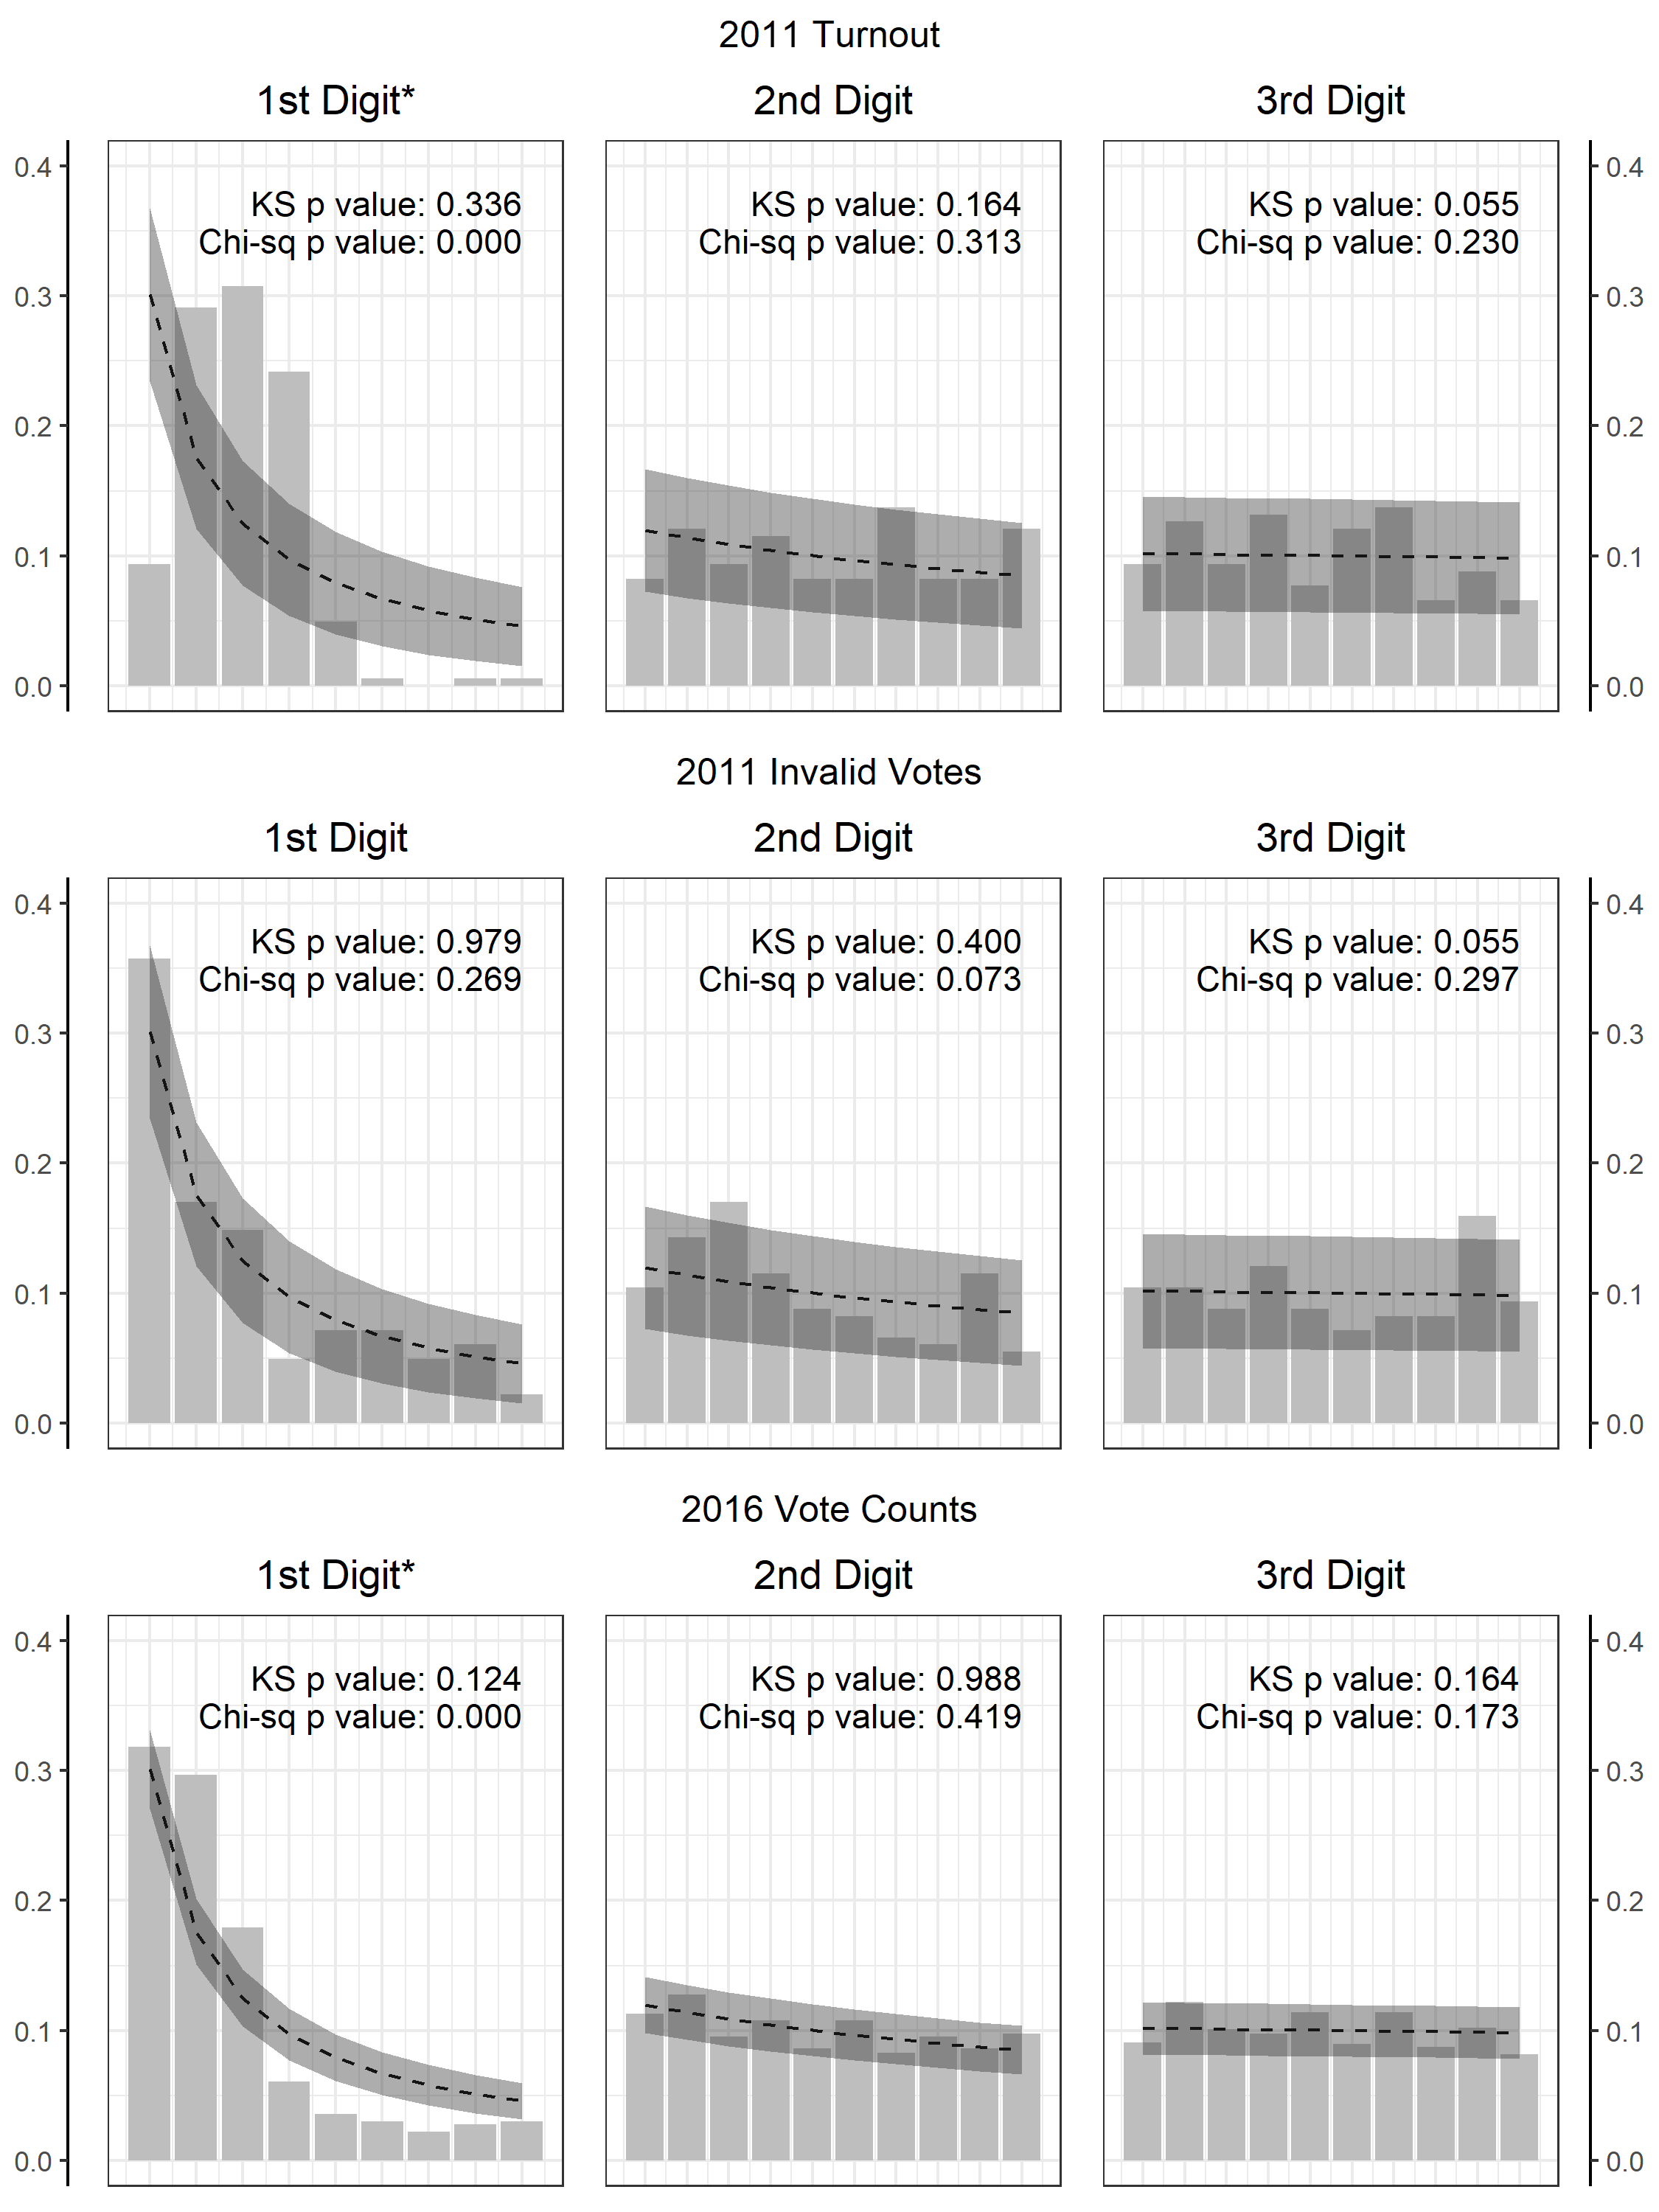
\includegraphics[height=.85\textheight]{figure/190916_digit_test.png}
	\caption[Digit Test of Election Results]{Empirical distribution (as bars) and expected distribution under Benford's Law (as dashed lines) of first, second, and third digits of district-level voter turnouts in the 2011 election, district-level invalid vote counts in the 2011 election, and candidate-level vote counts in the 2016 election. Shaded regions denote 95\% confidence intervals around the expected distributions. The first digits of 2011 turnout and 2016 vote counts (highlighted with \textsf{*}) are expected to violate Benford's Law even without tampering.}
	\label{fig:Benford}
\end{figure}

\clearpage

\section{Effect of 2015 State Budget Law}
\label{app:budget_law}

In 2015, the Vietnamese government issued a revised Law on the State Budget (hereafter 2015 State Budget Law), which became effective from the 2017 fiscal year onward. Among other changes, the revised law reiterated the centrality of the central government budget in fiscal governance i.e. fiscal recentralization \citep{Vu2016}. Practically, it led to major adjustments to provincial budgets, particularly through changes in the sharing rates--the proportions of shared revenues that provinces have to remit back to the central government (recall that the revenue generated into each province can be divided into two categories: revenues that belong to the province exclusively and revenues that must be shared between the provincial and the central government according to a fixed ratio). \autoref{tab:2015_budget_law_changes} lists out provinces that were impacted by these adjustments, along with the proportions of the shared revenues they get to keep, before and after the adjustments.

\begin{table}[!htp]
	\caption{Changes to the proportions that individual provinces get to keep out of revenue sources designated as shared revenues. Adapted from \textcite{BaoViet2016} with updated data from the Vietnamese Ministry of Finance.}
	\label{tab:2015_budget_law_changes} 
	\centering
	
		\begin{tabular}{@{}lccll@{}}
			\\[-1.8ex] 
			\hline
			\hline
			\\[-1.8ex]
			&
			\multicolumn{1}{c}{\begin{tabular}[c]{@{}c@{}}2011-2016\\ proportions\end{tabular}} &
			\multicolumn{1}{c}{\begin{tabular}[c]{@{}c@{}}2017-2020\\ proportions\end{tabular}} &
			\multicolumn{1}{c}{\begin{tabular}[c]{@{}c@{}}Close \\ defeat(s)?\end{tabular}} &
			\multicolumn{1}{c}{\begin{tabular}[c]{@{}c@{}}Close \\ victor(ies)?\end{tabular}} \\ \midrule
			Ho Chi Minh City & .23 & .18 & \multicolumn{1}{c}{\checkmark} & \multicolumn{1}{c}{\checkmark} \\
			Binh Duong       & .40 & .36 & \multicolumn{1}{c}{}  & \multicolumn{1}{c}{\checkmark} \\
			Ha Noi           & .42 & .35 & \multicolumn{1}{c}{\checkmark} & \multicolumn{1}{c}{\checkmark} \\
			Ba Ria-Vung Tau  & .44 & .64 &                       &                       \\
			Dong Nai         & .51 & .47 &                       &                       \\
			Vinh Phuc        & .60 & .53 &                       &                       \\
			Quang Ngai       & .61 & .88 &                       &                       \\
			Quang Ninh       & .70 & .65 &                       &                       \\
			Khanh Hoa        & .77 & .72 &                       &                       \\
			Da Nang          & .85 & .68 &                       &                       \\
			Hai Phong        & .88 & .78 &                       &                       \\
			Bac Ninh         & .93 & .83 &                       &                       \\
			Quang Nam        & 1   & .90 &                       &                       \\
			Hung Yen         & 1   & .93 &                       &                       \\
			Hai Duong        & 1   & .98 &                       &                       \\ 
			\\[-1.8ex] 
			\hline
			\hline
			\\[-1.8ex]
		\end{tabular}
	
\end{table}

Because the changes to the proportions became effective in 2017, the same year that budgetary responses to localized defeats are expected to take place, they may confound the main results of the paper. Specifically, because the changes mostly result in more productive provinces having to surrender a larger share of their revenues to the central government (with the exception of Ba Ria-Vung Tau and Quang Ngai, where oil-based revenues have been hit by falling prices), and because \autoref{tab:balance} in the main manuscript indicates that these provinces are more likely to experience central candidate defeats (this difference is not statistically significant, nonetheless), the confounding may lead to an upward bias in the effect estimates.

However, the confounding does not compromise any of the main findings because there is little overlap between the provinces affected by the 2015 State Budget Law and those included in my samples. Columns 4 and 5 of \autoref{tab:2015_budget_law_changes} list out which of the former group of provinces have encountered close central candidate defeats or victories in the 2016 election. With the exception of Ha Noi and Ho Chi Minh City, which are already excluded from analysis for other reasons, Binh Duong remains the only province for which the confounding could manifest. Given the province's sizable economy, which makes it a likely influential outlier, prudence suggests that I exclude it from the main analysis.

With Binh Duong excluded from the sample, the main effect estimates should no longer be confounded by budgetary changes following the 2015 State Budget Law. They remain consistently positive and statistically significant, confirming that the findings are not driven by the effect of the 2015 State Budget Law. When compared with an analysis that includes Binh Duong, the point estimates for the linear fixed effects models are smaller, suggesting that the risk of confounding is indeed non-trivial and the exclusion of Binh Duong indeed leads to more conservative results. Reassuringly, the sample without Binh Duong still exhibits balance in terms of both pre-treatment covariates and pre-treatment outcomes.

\clearpage

\section{Robustness to small sample size}
\label{app:small_sample}

One potential issue with the analysis in the main manuscript is that it leverages a relatively small sample size, particularly for the treated group. A small sample size typically undermines an analysis in two ways: it a) leads to incorrect inferences when the inferential techniques depend on large sample asymptotic properties and b) generates unreliable estimates because even small variations in the composition of control and treatment groups occurring both randomly or due to coding or measurement errors could have led to very different estimates. I show, however, that neither of these problems should invalidate the findings in the main manuscript.

In terms of inferences, because the sample of treated units in the analysis is close to the universe of all treated provinces in Vietnam, it approximates a finite sample. In this case, methods using exact tests through randomization inference should be adequate because they do not depend on asymptotic properties that only work with larger samples.

In terms of estimate reliability, the original estimates are fairly robust to variation in the sample, meaning that even if the composition of the control and treatment groups had been different the analysis would have reached the same conclusion. I verify this robustness with a jackknife approach. Specifically, I introduce perturbations in the sample through four procedures: adding back the one province that was excluded from the treatment group because it experienced only a heavy defeat (Soc Trang), dropping one treatment province at a time, adding one province from those that saw neither defeats (of any kind) nor close wins to the control provinces at a time, and dropping one control province at a time. For each procedure, I re-estimate the main results using linear fixed effects models for every resulting perturbed sample and compare the new results with the original estimates in the main manuscript.

\begin{figure}[!htbp]
	\centering
	\begin{subfigure}{.8\textwidth}
		\centering
		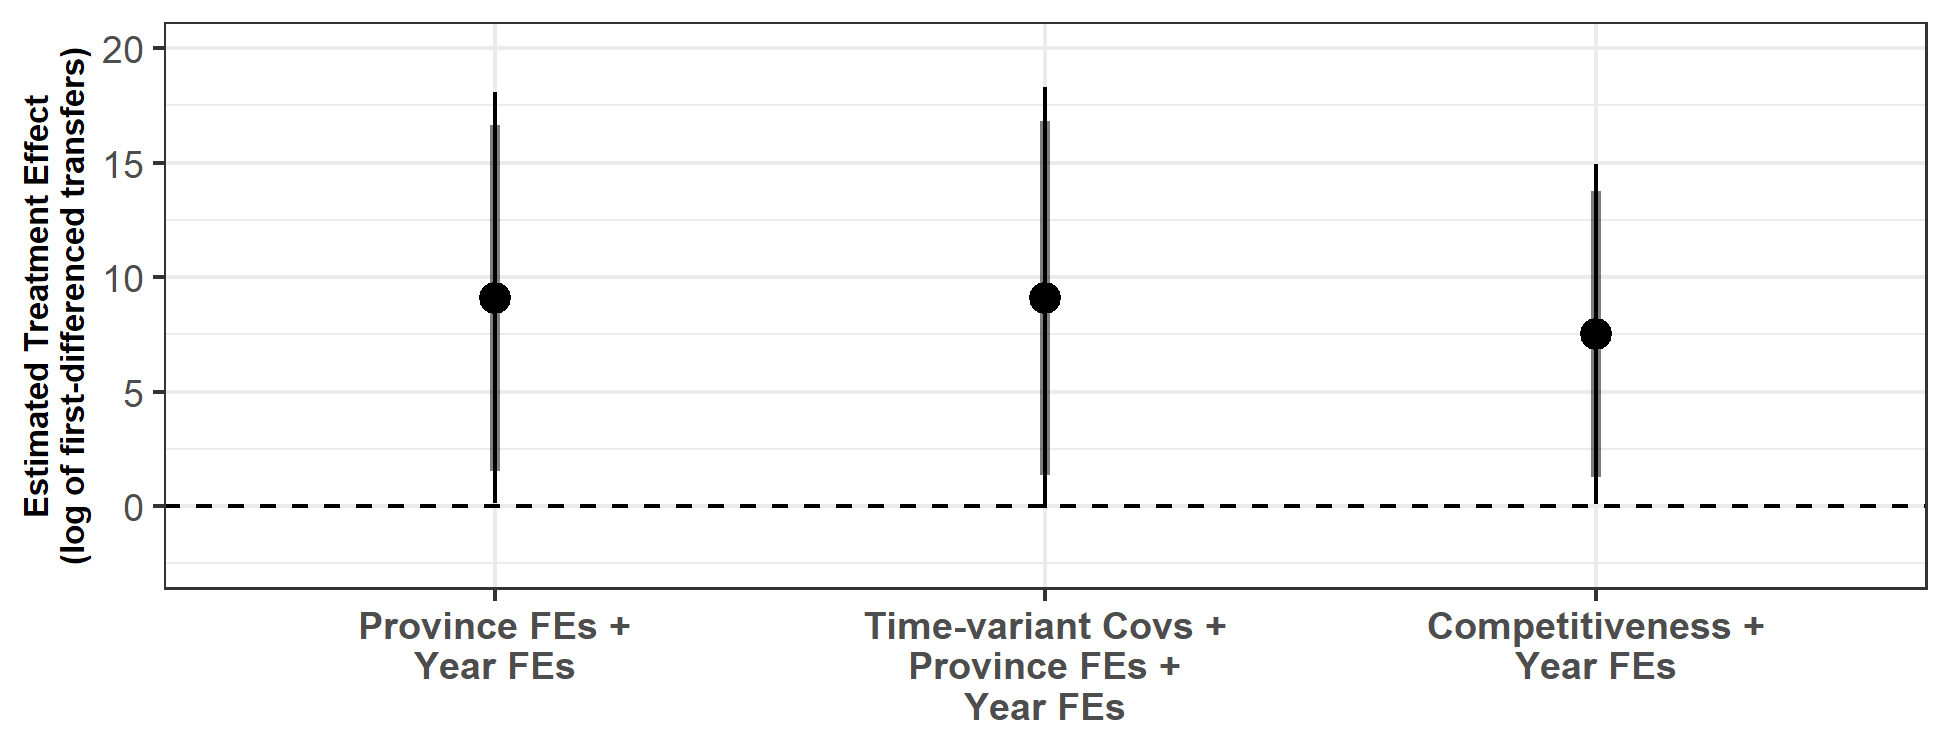
\includegraphics[width=\textwidth]{figure/210202_perturb_results_treat_add.png}
		\captionsetup{singlelinecheck=off, justification=centering}
		\caption{Adding Soc Trang back to treated group}
	\end{subfigure}
	\begin{subfigure}{.8\textwidth}
		\centering
		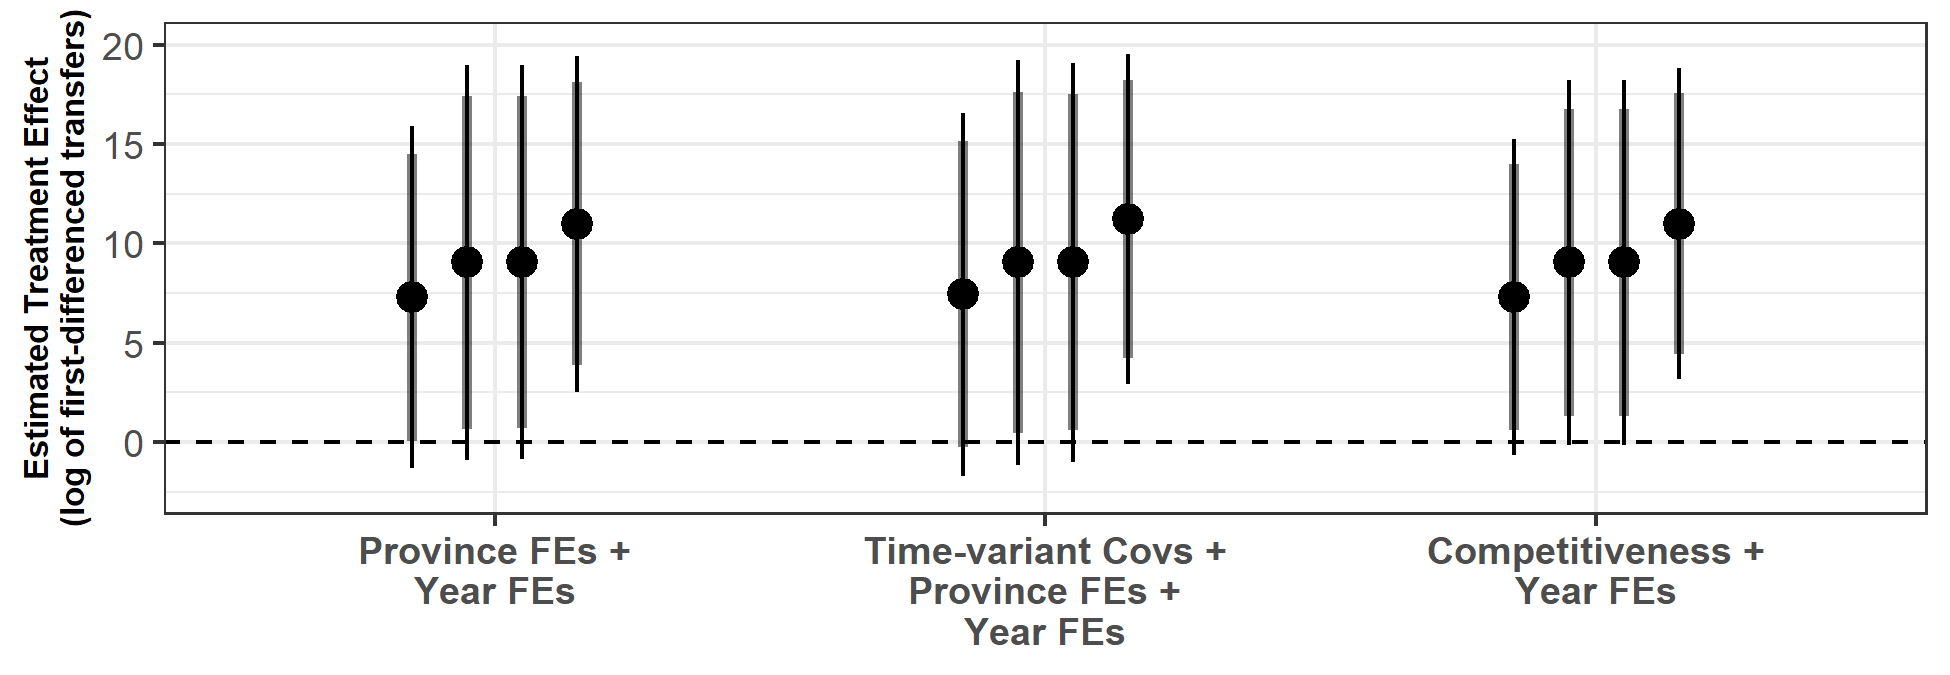
\includegraphics[width=\textwidth]{figure/210202_perturb_results_treat_drop.png}
		\captionsetup{singlelinecheck=off, justification=centering}
		\caption{Dropping one treated province}
	\end{subfigure}
	\begin{subfigure}{.8\textwidth}
		\centering
		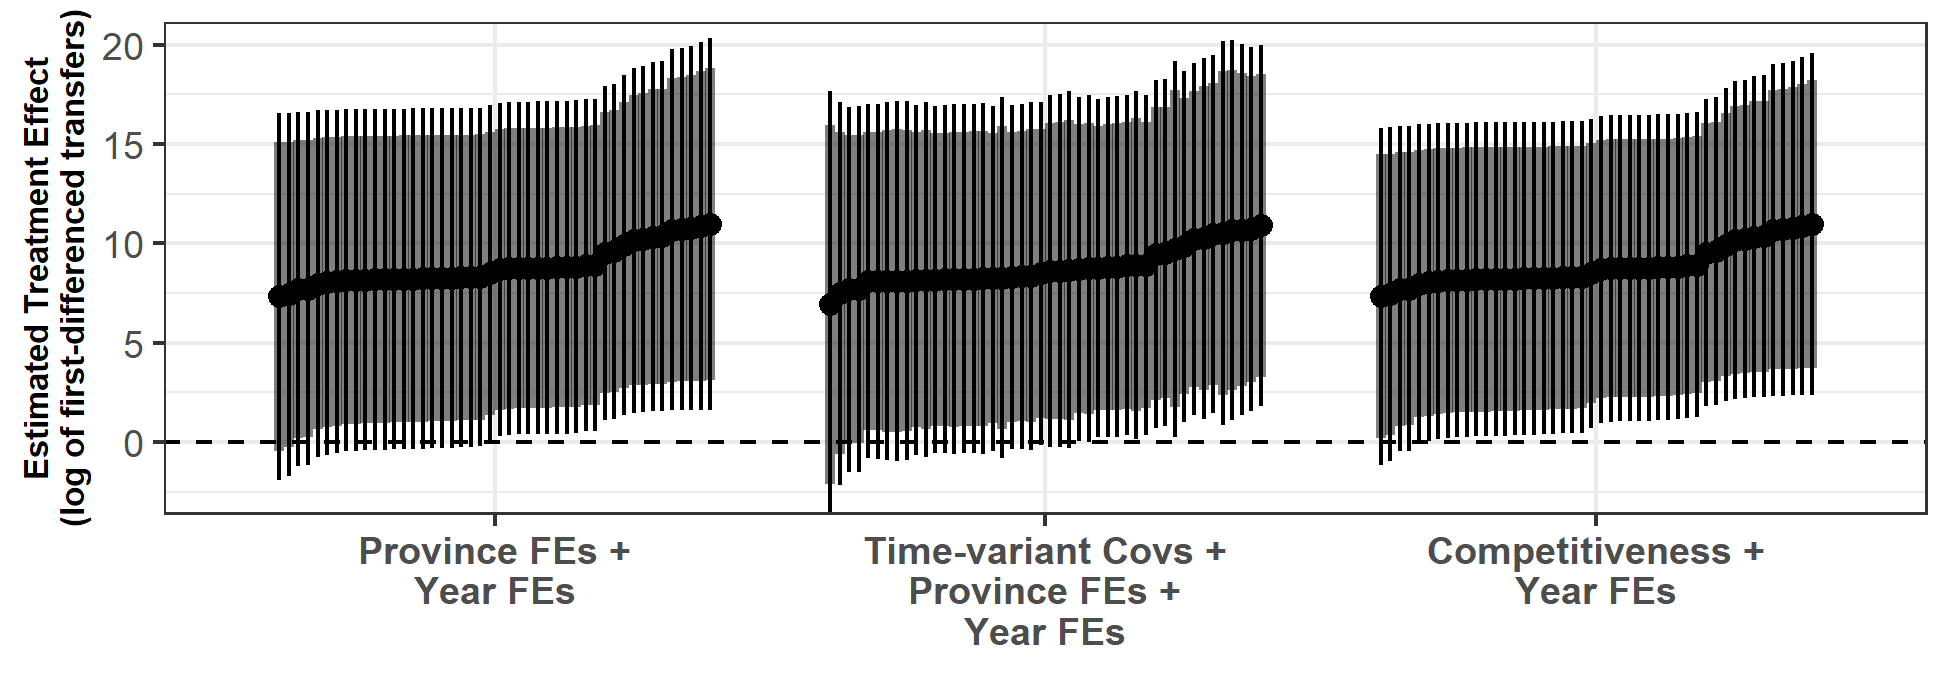
\includegraphics[width=\textwidth]{figure/210202_perturb_results_control_add.png}
		\captionsetup{singlelinecheck=off, justification=centering}
		\caption{Adding one control province}
	\end{subfigure}
	\begin{subfigure}{.8\textwidth}
		\centering
		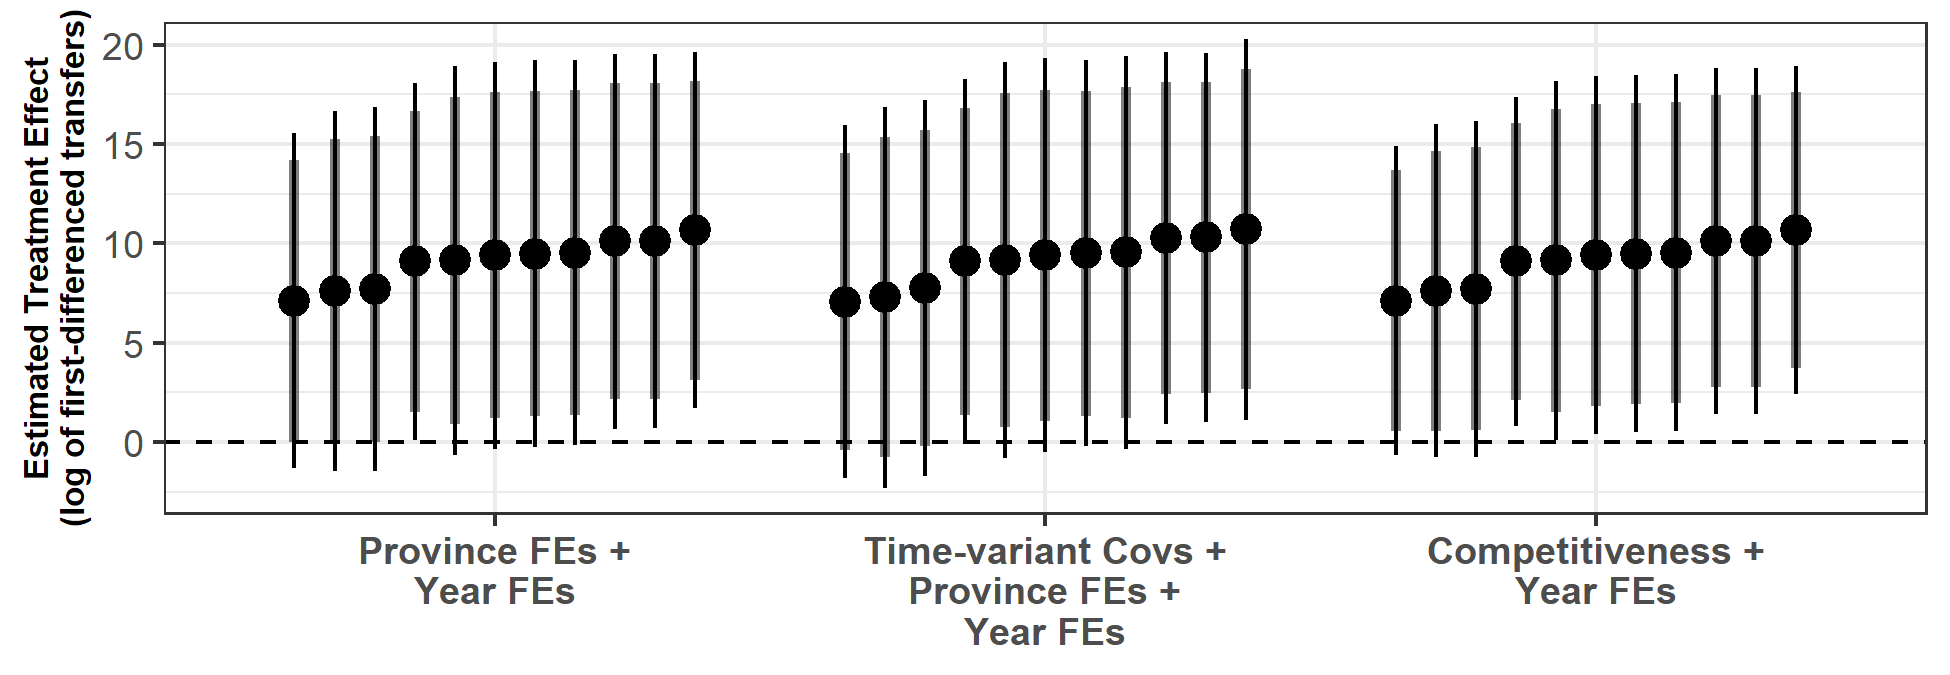
\includegraphics[width=\textwidth]{figure/210202_perturb_results_control_drop.png}
		\captionsetup{singlelinecheck=off, justification=centering}
		\caption{Dropping one control province}
	\end{subfigure}
	\caption[Estimated linear fixed effects treatment effects on log of first-differenced central transfers for perturbed samples]{Estimates of instantaneous treatment effects using linear fixed effects models on perturbed samples under different perturbation procedures. Thick error bars show 90\% confidence intervals and thin error bars show 95\% confidence intervals.}
	\label{fig:lfe_perturb}
\end{figure}

The distributions of instantaneous treatment effects estimated using the perturbed samples are plotted separately for each perturbation procedure in \autoref{fig:lfe_perturb}. In every plot, all the point estimates are close to each other--and to the original estimates--suggesting that they are not sensitive to perturbations to the sample. Although the procedure adds noise, nearly all the estimates are found to be statistically significant, with the majority being significant at the .05 level and nearly all remaining estimates being significant at the .1 level. Even more reassuringly, all but a couple of  estimates for the persistent treatment effects (not shown here) are significant at the .05 level. This confirms that the main findings are unlikely to be artifacts of the specific sample and the specific composition of control and treated provinces in the data. 

\clearpage 

\section{Robustness outside of close elections}
\label{app:bandwidth}

\begin{table}[!h]

\caption{\label{tab:candidates_stats}Summary of candidate-level statistics for central candidates 
      within different ranges of vote margins. Standard errors appear in parentheses.}
\centering
\begin{tabular}[t]{>{\raggedright\arraybackslash}p{10em}>{\centering\arraybackslash}p{4.1em}>{\centering\arraybackslash}p{4.1em}>{\centering\arraybackslash}p{4.1em}c}
\toprule
\multicolumn{1}{c}{ } & \multicolumn{4}{c}{Vote Margin} \\
  & (-30,-10] & (-10,10] & (10,30] & (30,50]\\
\midrule
\addlinespace[.5em]
\multicolumn{5}{l}{\textbf{Including Hanoi, Ho Chi Minh City, and Binh Duong}}\\
N & 5 & 35 & 96 & 61\\
Age & 60.40 & 54.69 & 52.44 & 55.54\\
 & (3.49) & (1.43) & (0.65) & (0.72)\\
Male & 1 & 0.94 & 0.81 & 0.87\\
 &  & (0.04) & (0.04) & (0.04)\\
CPV Member & 1 & 0.89 & 0.97 & 0.98\\
 &  & (0.05) & (0.02) & \vphantom{1} (0.02)\\
Years in CPV & 34.00 & 25.94 & 26.14 & 29.22\\
 & (5.37) & (1.38) & (0.91) & (1.11)\\
Education Level (1-5) & 2.60 & 3.54 & 3.21 & 3.28\\
 & (0.40) & (0.19) & (0.09) & (0.14)\\
Power Index (1-5) & 1 & 1.60 & 2.02 & 2.54\\
 &  & (0.11) & (0.08) & (0.14)\\
\addlinespace[.5em]
\multicolumn{5}{l}{\textbf{Excluding Hanoi, Ho Chi Minh City, and Binh Duong}}\\
N & 1 & 19 & 86 & 60\\
Age & 52.00 & 53.89 & 52.21 & 55.27\\
 &  & (1.53) & (0.67) & (0.68)\\
Male & 1 & 0.89 & 0.83 & 0.87\\
 &  & (0.07) & (0.04) & (0.04)\\
CPV Member & 1 & 0.95 & 0.98 & 0.98\\
 &  & (0.05) & (0.02) & (0.02)\\
Years in CPV & 24.00 & 25.33 & 25.62 & 28.88\\
 &  & (1.81) & (0.94) & (1.08)\\
Education Level (1-5) & 3.00 & 3.53 & 3.21 & 3.23\\
 &  & (0.22) & (0.09) & (0.14)\\
Power Index (1-5) & 1 & 1.63 & 2.03 & 2.52\\
 &  & (0.16) & (0.08) & (0.14)\\
\bottomrule
\end{tabular}
\end{table}



% Table created by stargazer v.5.2.2 by Marek Hlavac, Harvard University. E-mail: hlavac at fas.harvard.edu
% Date and time: Mon, Jan 25, 2021 - 5:33:05 PM
\begin{table}[!htbp] \centering 
  \caption{Estimated treatment effects of localized defeats on log of first-differenced central transfers 
          from linear fixed effects models for a full sample without restriction on central candidate vote margins.} 
  \label{tab:lfe_simple} 
\begin{tabular}{@{\extracolsep{5pt}}lcccccc} 
\\[-1.8ex]\hline 
\hline \\[-1.8ex] 
 & \multicolumn{3}{c}{Instantaneous Effect} & \multicolumn{3}{c}{Persistent Effect} \\ 
\\[-1.8ex] & (1) & (2) & (3) & (4) & (5) & (6)\\ 
\hline \\[-1.8ex] 
 Treatment Effect & 6.901$^{**}$ & 6.590$^{**}$ & 6.901$^{***}$ & 5.737$^{***}$ & 5.194$^{***}$ & 5.737$^{***}$ \\ 
  & (2.770) & (2.891) & (2.494) & (1.706) & (1.896) & (1.587) \\ 
 \hline \\[-1.8ex] 
Election Competitiveness &  &  & Yes &  &  & Yes \\ 
Time-variant Covariates &  & Yes &  &  & Yes &  \\ 
Province FEs & Yes & Yes &  & Yes & Yes &  \\ 
Year FEs & Yes & Yes & Yes & Yes & Yes & Yes \\ 
\hline \\[-1.8ex] 
N & 300 & 300 & 300 & 420 & 420 & 420 \\ 
R$^{2}$ & 0.489 & 0.503 & 0.319 & 0.410 & 0.427 & 0.261 \\ 
\hline 
\hline \\[-1.8ex] 
\multicolumn{7}{l}{$^{*}$p $<$ .1; $^{**}$p $<$ .05; $^{***}$p $<$ .01} \\ 
\end{tabular} 
\end{table} 


\begin{figure}[!htbp]
	\centering
	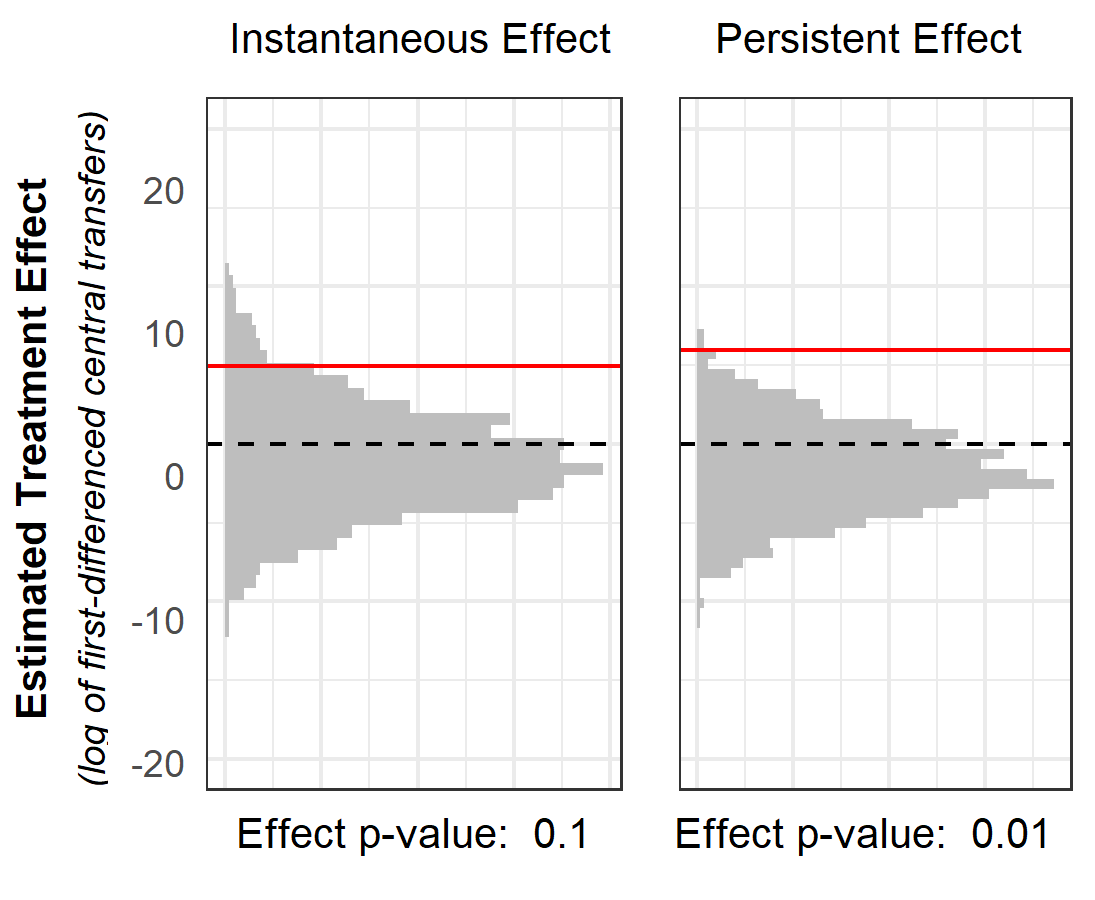
\includegraphics[]{figure/210202_rdd_simple_results.png}
	\captionsetup{singlelinecheck=off}
	\caption[Estimated RDD treatment effects]{Estimates of treatment effects on log of first-differenced central transfers from RDD analyses using the local randomization approach on the full sample without central candidate vote share restrictions. The red lines show the estimated treatment effects, and the gray bars show their randomization distribution. P-values are presented for the treatment effect estimate.}
	\label{fig:rdd_simple}
\end{figure}

\begin{figure}[!htbp]
	\centering
	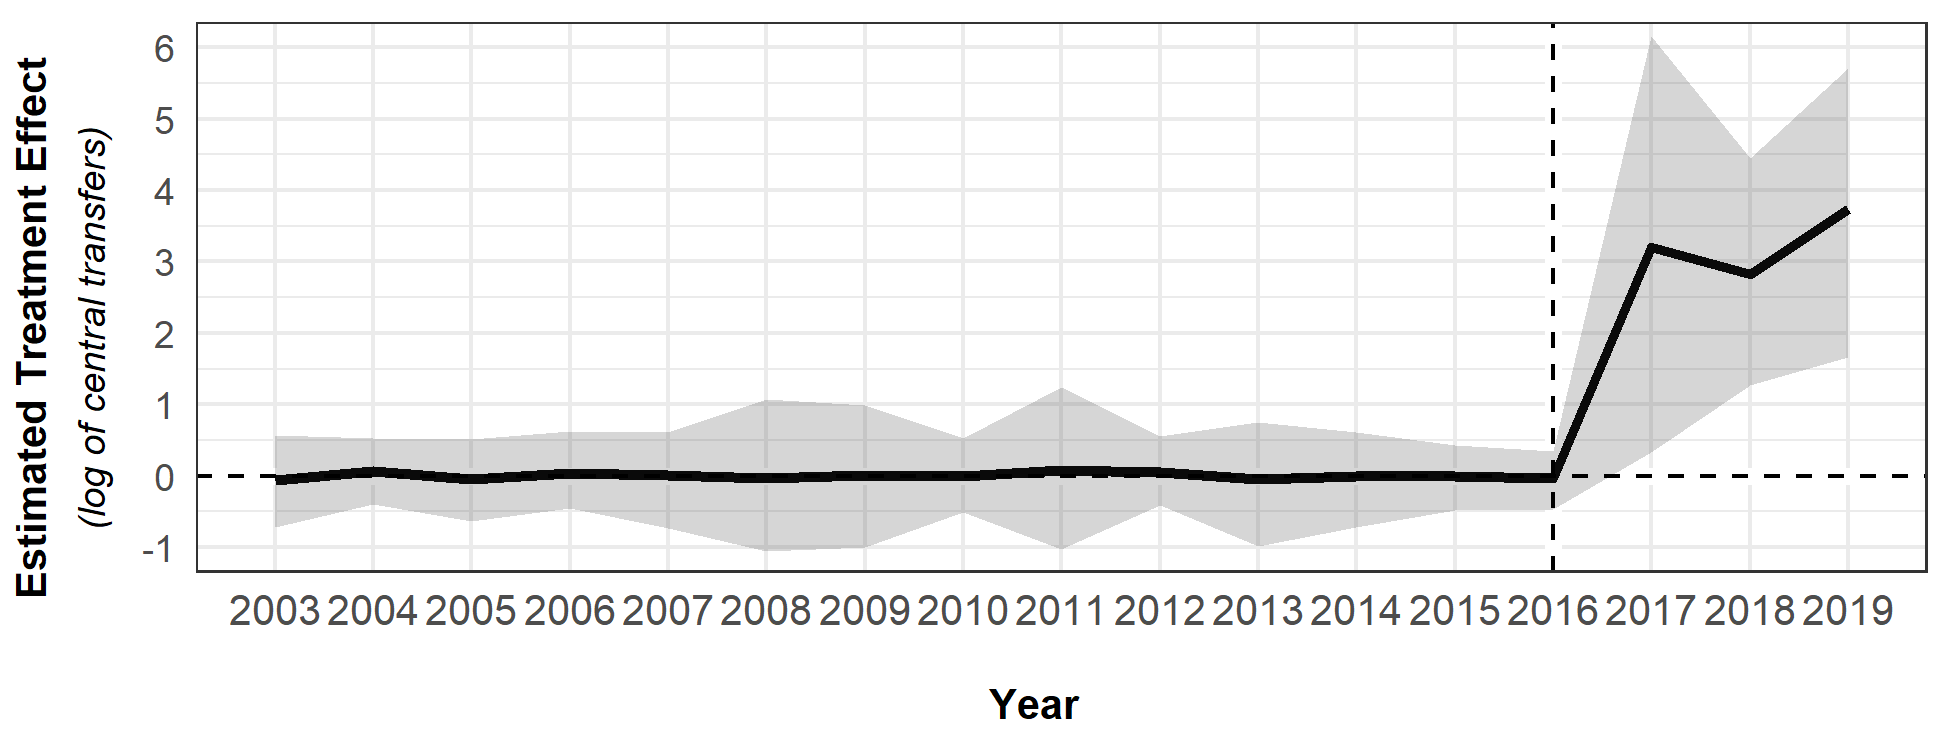
\includegraphics[width=\textwidth]{figure/210125_synth_simple_results.png}
	\captionsetup{singlelinecheck=off}
	\caption[Estimated synthetic control treatment effects]{Estimates of treatment effects on log of central transfers using the generalized synthetic control method on the full sample without central candidate vote margin restrictions. They gray region represents 95\% confidence interval obtained by the parametric bootstrap. The vertical dashed line marks the election year.}
	\label{fig:synth_simple}
\end{figure}


\clearpage
\section{Findings from previous elections}
\label{app:previous_elections}

\subsection{Why focus on the 2016 election?}

The main manuscript focuses on the 2016 election to achieve the maximum inferential leverage. Compared to previous elections in 2007 and 2011,\fnote{Data from elections before 2007 are not available.} the 2016 election offers more valuable data in two ways. First, only in 2016 did the CPV include vote shares for defeated candidates when releasing election results. Official result releases in previous elections only listed out the names and vote shares of elected candidates, along with district-level statistics such as turnout. Although defeated candidates can still be identified by comparing the pre-election candidate list with the final results, it is impossible to determine the margin by which each of them has lost. 

Information about margins is important because it helps separate out central candidate defeats that were close and hence informative from defeats that seemed too certain to contain new information. Central candidates who lost by large margins are likely to be different from those who lost only narrowly, and provinces in which heavy defeats happened are also likely to be different. At the candidate level, heavy losers may be unpopular with both the voting public and the provincial Party apparatus. Although unlikely, they may also be ``undesirable'' elites that the ruling party wishes to punish by forcing to contest an unwinnable election. At the province level, heavy defeats are more likely to signal blatant acts of resistance by provincial officials, acts that could only be expected from the most defiant provinces, which are also likely to be those most financially independent of the central government. In each of these scenarios, what sets the candidates or the provinces apart--the candidates' unpopularity or the provinces' defiance--must be serious enough that it cannot go unnoticed. In other words, when heavy defeats happen, the central leadership is likely to already know the underlying causes. Unlike close defeats which may have surprised the CPV, heavy defeats thus bring less information content and are less likely to elicit the same kind of response. Including these defeats in the analysis would lead to no new insights about how the regime acquires and reacts to new information from elections and in practice may lead to biased estimates.

Specifically, bias induced by the uniqueness of heavy defeats could manifest in two different ways. Firstly, if these defeats were not surprising and thus did not induce any reaction by the regime, then an estimate of their ``treatment effect'' would likely be zero, which would then bias the average treatment effect estimate downwards. Conversely, if heavy defeats actually indicated successful attempts by provincial officials to punish undesirable elites on behalf of the regime, then estimates of the average treatment effect would be inflated by any budgetary rewards that the provinces may receive for such successes. Secondly and more importantly, if heavy defeats reflected a high degree of independence by the provinces, then both the level of central transfers these provinces received in the election year, as well as the year-to-year changes over preceding years, would likely be different. The result is the problem of dynamic causality \parencite{ImaiKim2019}, occurring because past central transfers are almost certainly determinants of present central candidate defeats. Because provinces with heavy defeats differ from provinces with no defeats both in the level of potential outcomes as well as the probability of experiencing defeats, the difference in post-election central transfers between these sets of provinces no longer reflects a true, unbiased treatment effect of localized defeats. In other words, even if the central government also adjusted central transfers to these provinces in response to the heavy defeats, an estimate based on these provinces would still be biased by other confounders unrelated to the treatment of interest. 

Thus, the selection strategy using close victories and defeats is necessary because it ensures that the estimated changes in central transfers are attributed to information from the defeats alone. For 2016, only one central candidate defeat was heavy enough to be excluded under this selection strategy, but there is no guarantee that heavy central candidate defeats had been similarly rare in 2011 and 2007. On the contrary, as my analysis later in this section will show, attempts to separate heavy defeats from close ones using information on vote shares yield large variations in treatment effect estimates, suggesting that confounding is serious for these two past elections.

Additionally, margins are also necessary in determining the close wins that would form the control group. Even though vote shares for central candidates who won are known, the margins by which they won cannot be determined without the vote share of the defeated candidates immediately behind them in the race. Because the vote shares of defeated candidates vary and may even exceed 50\%, using thresholds based on winners' vote shares alone may easily lead to false negatives. Indeed, in the 2016 election, 7 out of 15 close central candidate victories were won with winners' vote shares above 60\%, such that using this threshold to identify close wins would have caused 5 provinces to incorrectly drop out of the control set. This would have resulted in a loss in precision.

The second benefit of focusing on the 2016 election is that it offers a longer pre-treatment period for the generalized synthetic control method \citep{Xu2017gsynth}. Given that budgetary data for Vietnam is only available from 2003, an analysis that on the 2016 election and hence designating 2017 as the first post-treatment year will have 14 pre-treatment years, much closer to \citepos{Abadie2010} recommendation than the 9 pre-treatment years available for an analysis focused on the 2011 election. The longer pre-treatment period allows more data to go into the construction of the synthetic controls, which in turn leads to a more inferentially valid comparison. In addition, the synthetic control constructed from thinner data is less likely to perfectly match treated observations' outcome history and thus less effective at tackling dynamic causality.

When the sample is dynamically balanced like in the main analysis, inferences using the generalized synthetic control method are unlikely to diverge from linear fixed effects models and thus function primarily to further validate these results. When there is significant threat of dynamic causality, however, the generalized synthetic control method is the only way to mitigate this problem. Because the sample from the 2007 and 2011 elections is likely to suffer from dynamic causality but does not contain sufficient data for the generalized synthetic control method to perform optimally, the main analysis prioritizes data from the 2016 election to maximize internal validity.

\subsection{Responses to localized defeats in the 2011 election}

Even though focusing on the 2016 election would lead to the most internally valid inferences, external validity requires that I identify whether similar increases in central transfers can also be observed following localized defeats of central candidates in previous elections. I thus attempt to extend the main analysis in this paper to the 2011 and 2007 elections.

As discussed above, I anticipate several analytical challenges. For the linear fixed effects models, the lack of data on margins means that the resulting analysis will be restricted to the ``naive'' sample that counts all provinces with any central candidate defeat as treated and all provinces with central candidate winning with less than 60 percent vote share as control. In other words, I am likely to over-count treated provinces and under-count control provinces. This is expected to result in important pre-treatment dissimilarity between treated and control provinces as well as weaker precision. Although the models' inferences are only valid for provinces with narrow central candidate victories and defeats, the 2011 treated pool also contains an unknown number of provinces with only heavy defeats. Because these provinces are not comparable to provinces with close central candidate victories, estimates of the treatment effect are likely to be biased. \autoref{fig:lfe_placebo_2011}, which plots estimates of the persistent treatment effect using the ``naive'' sample for the 2011 election against three placebo treatment effects estimated by assuming the 2011 election had instead happened in 2008, 2009, and 2010, confirms this concern. There are large placebo effects detected for 2009 and 2010, which should not be expected if treated and control provinces are comparable. The placebo effects for 2009 in particular are large in magnitude and are significant at the .05 level. Each placebo effect for 2011 is larger than the corresponding effect for 2016, suggesting serious dynamic imbalance with the ``naive'' sample. For this reason, the main effect estimates, which are positive but indistinguishable from zero, should not be considered as reliable.

\begin{figure}[!htbp]
	\centering
	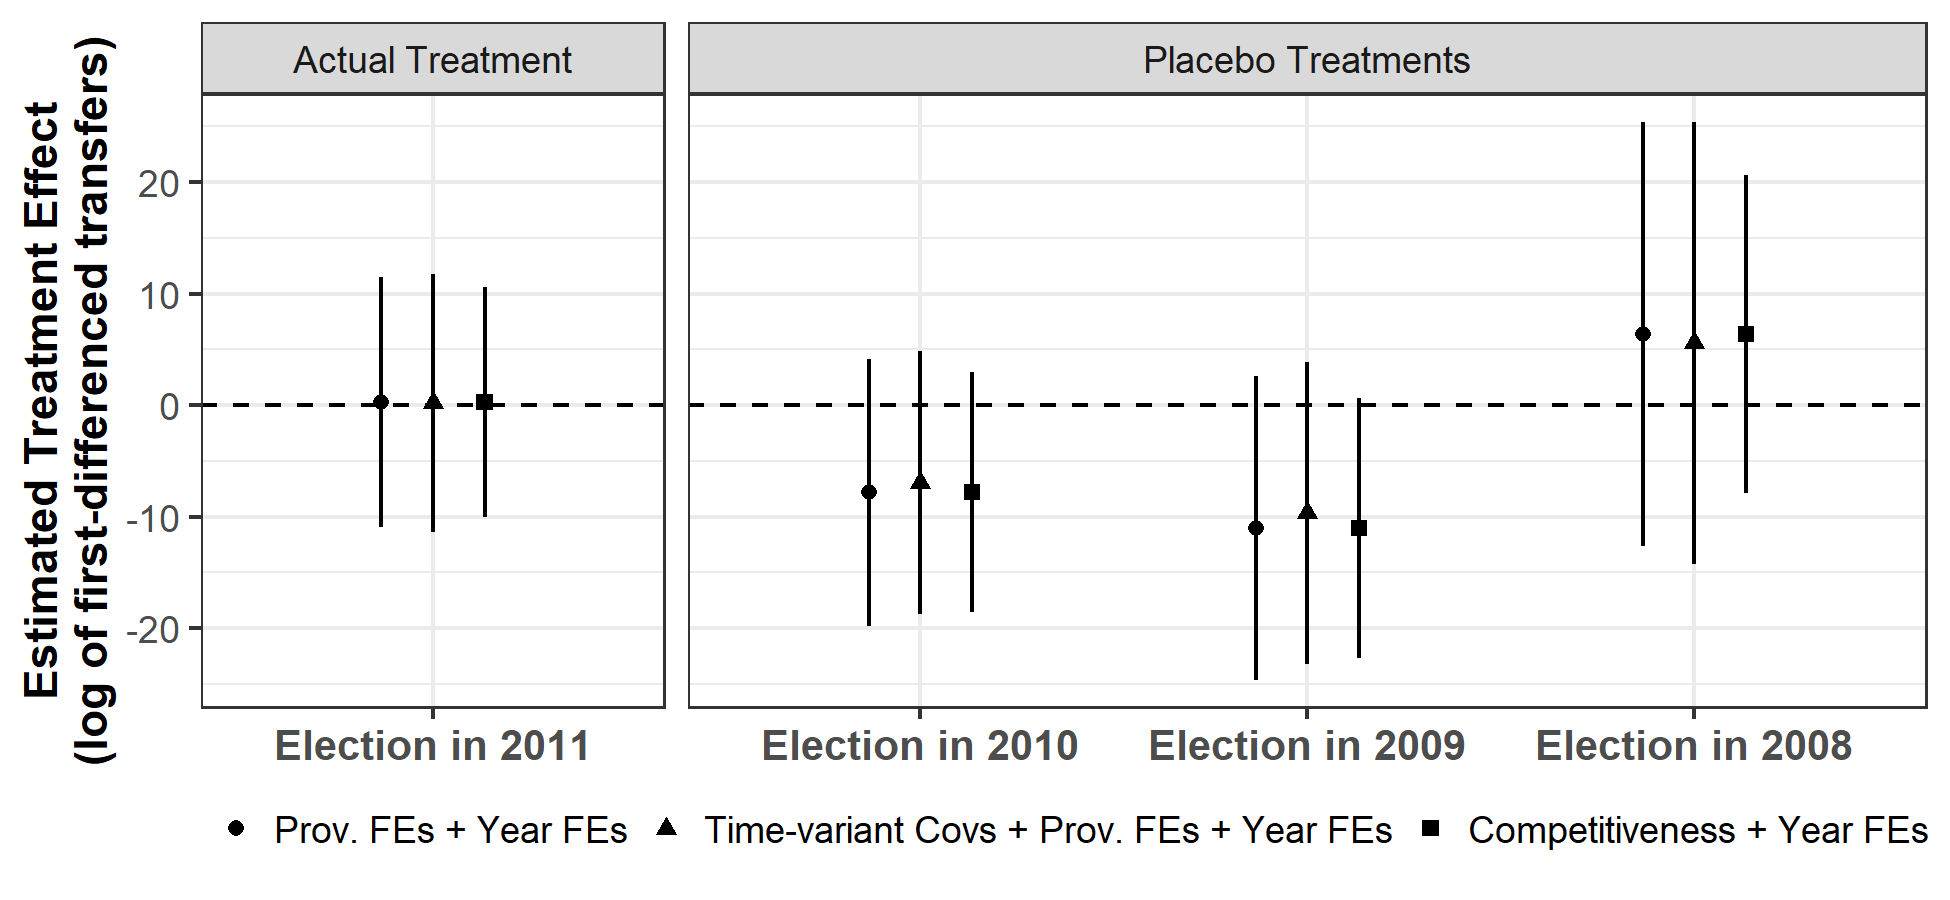
\includegraphics[]{figure/210202_lfe_placebo_2011.png}
	\captionsetup{singlelinecheck=off}
	\caption[Estimated placebo linear fixed effects treatment effects for 2011]{Estimates of persistent treatment effects on log of first-differenced central transfers for the 2011 election using linear fixed effects models. All central candidate defeats are included in the sample. Error bars show 95\% confidence intervals.}
	\label{fig:lfe_placebo_2011}
\end{figure}

To compound the problem, the candidate-level local randomization procedure is no longer appropriate for this case. Recall that this procedure involves identifying a window of vote margins, such that the results of central candidates who lost and won with margins within this window can be considered as-if random. Without vote share data from defeated candidates to calculate margins, no such window can be defined. The closest alternative is an one-sided window defined by an upper boundary on winners' vote shares, such that the sample would include all central candidates who won with vote shares smaller than this boundary. The resulting window, however, would still include all defeated central candidates, including those whose defeats are too severe to ever be considered as-if random. This undermines the logic of the regression discontinuity framework.

In light of the problem facing the linear fixed effects analysis and the inapplicability of the local randomization approach, the generalized synthetic control method \citep{Xu2017gsynth} becomes much more important. Compared to linear fixed effects model, it is more effective at addressing dynamic causality, even when it is unable to account for unobserved time-invariant confounders \autocite{ImaiKim2019}. Given the possibility of dynamic imbalance revealed in \autoref{fig:lfe_placebo_2011}, this method seems preferable for the 2011 analysis.

\autoref{fig:synth_results_2011} shows the result from an analysis applying the generalized synthetic control method \citep{Xu2017gsynth} to data from the 2011 election. Most importantly, it shows that estimates of localized defeats' treatment effect exhibit an initial drop, followed by an steady increase in the following years, with magnitude increasing the further away from the election year before dropping back to nearly zero in 2015 (the year before the next election). Despite the drops in 2012 and 2015, the average treatment effect calculated over all four post-election years is still positive and statistically significant at the .1 level. 

As evident in the much smaller placebo treatment effects at 2009, 2010, and 2011, the generalize synthetic control has mitigated pre-treatment differences in net transfers between treated and control provinces. When compared with results from the linear fixed effects, it is possible to see that the magnitude of the treatment effect increases as dynamic imbalance is reduced, suggesting that the confounding induced by dynamic causality may have led to a downward bias. In any case, the evidence from this analysis, though tentative, does suggest a positive effect i.e. an increase in central transfers to provinces that experienced localized defeats.

\begin{figure}[!h]
	\centering
	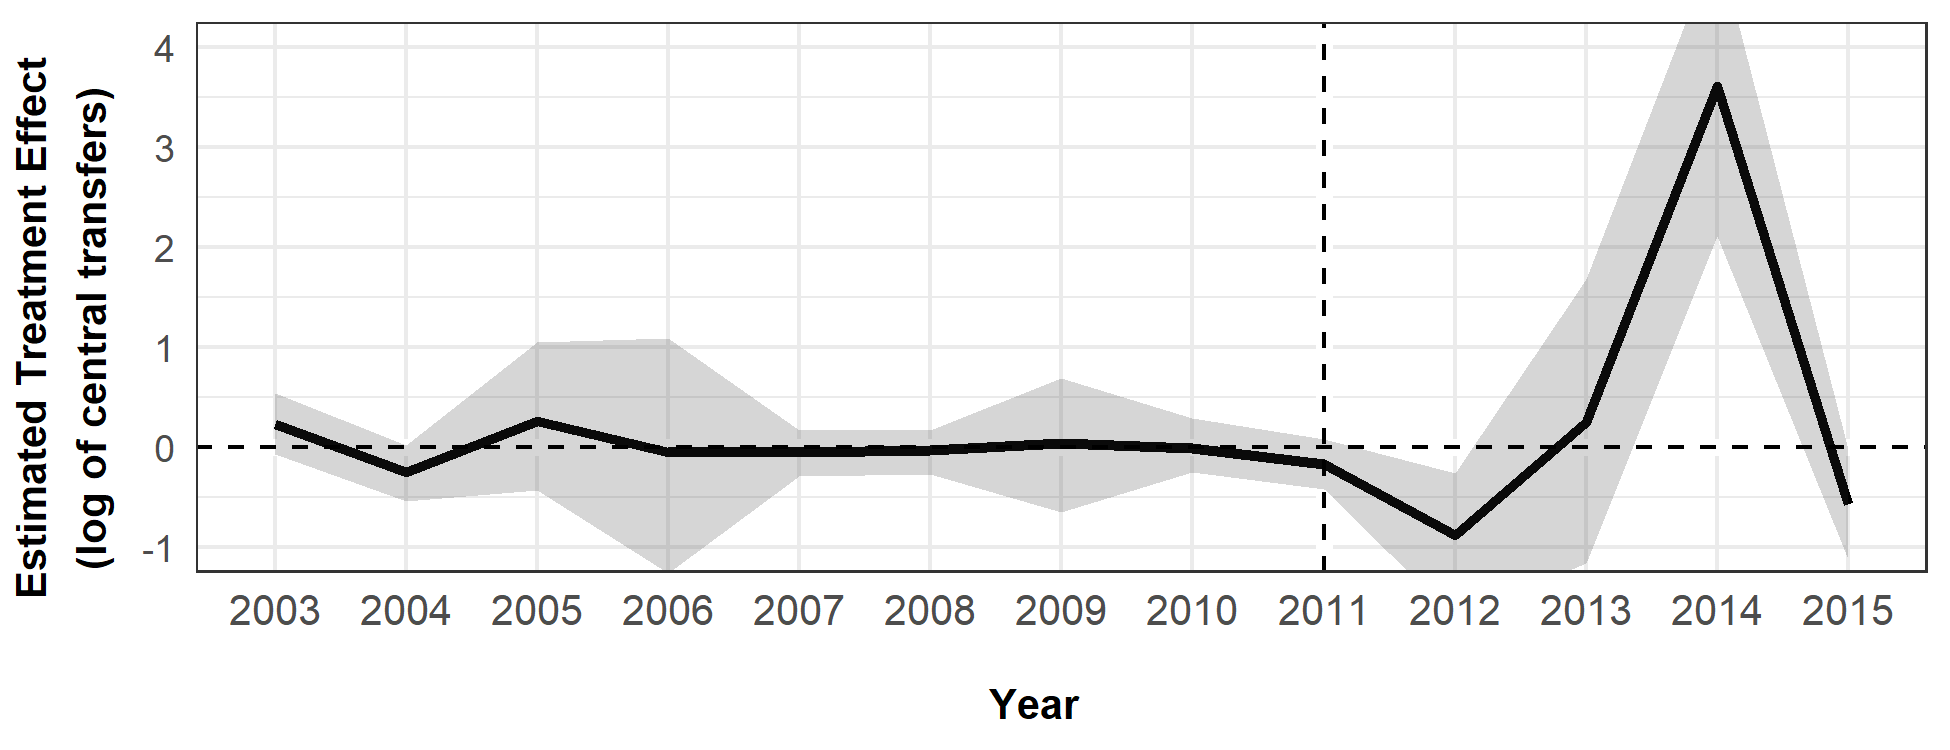
\includegraphics[]{figure/210202_synth_results_2011.png}
	\captionsetup{singlelinecheck=off}
	\caption[Estimated synthetic control treatment effects for 2011]{Estimates of treatment effects for the 2011 election using the generalized synthetic control method. All central candidate defeats are included in the sample. The horizontal dashed line marks the election year.}
	\label{fig:synth_results_2011}
\end{figure}

To confirm that the positive treatment effect identified by the generalized synthetic control method \citep{Xu2017gsynth} is indeed appropriate and not the result of unprincipled cherry-picking, I show that this result is achievable with linear fixed effects models if cases of close victories and defeats could be identified. To do this, I use available data on winning candidates' vote shares to simulate a large number of educated guesses about defeated candidates' performance, construct indicators of central candidates' close victories and defeats based on these guesses and then estimate plausible treatment effects based on these indicators. The distribution of estimates obtained from this exercise will then cover the ``true'' treatment effects that would have been identified when all data is available.

Educated guesses about defeated candidates' vote shares are possible because these shares are not completely unknowable. Because Vietnam's electoral rules specify that each voter gets to vote for as many candidates as there are seats in the district, the maximum value of the sum of all candidates' vote shares in the districts is 100 percent times the number of seats. For example, in a district with five candidates and three seats, the sum of all five candidates' vote shares must not exceed 300 percent. For each district, the sum of all the losers' vote shares must not exceed the difference between this maximum sum and the sum of all the winners' vote shares--data for which is available. In addition, each individual loser's vote share cannot exceed that of the lowest winning candidate (or, in districts with unfilled seats, the 50-percent threshold). Altogether, these facts limit the range within which each defeated candidate's vote share could lie.

Given the above limit, I simulate possible values for all the defeated central candidates by randomly allocating the ``left-over'' vote shares that did not belong to the winning candidates in each districts among the losers, leaving aside a small share representing unallocated votes from voters who did not use up all their votes or those who voted for write-in candidates. Specifically, for each district with $k$ defeated candidates, I draw random samples of proportions from the constrained $(k+1)$-simplex, with the constraints defined by the maximum vote share a defeated candidate could secure as well as an upper limit of .1 on the share of unallocated votes and distribute the ``left-over'' vote shares according to these proportions.\fnote{The constraint on unallocated vote shares is based on the expectation that votes rarely go unallocated and on the observed distribution of these votes in the 2016 election}\fnote{A probability simplex is a vector of probability $p_1, p_2, \dots, p_k$ such that $\sum_{k}^{i=1}p_i = 1$. Random samples from the simplex are drawn using the Dirichlet distribution. To avoid making assumptions about the relative distribution of vote shares among defeated candidates, I draw from the uniform Dirichlet distribution with $\mathbf{\alpha} = \mathbf{1}$ and enforce the constraints with rejection sampling. A more efficient method is to draw from a distribution with $\alpha_i > 1$, but this assumes that highly unequal distribution of votes among defeated candidates are unlikely. Yet another method is to model the shape parameters for each district based on observed data for 2016, which requires additional modeling assumptions. In practice, different sampling approaches yield very similar results.} With a large number of draws, the resulting distribution will approximate the universe of all possible values of the unobserved vote shares.

Then, taking each random allocation of vote shares as one hypothetical observation of the defeated candidates' vote shares, I calculate winning and losing margins for all central candidates and use these margins to construct district-level and province-level indicators of localized defeats. The resulting distribution of province-level treatment indicator vectors from this step provides the unconditional likelihood that each province has experienced narrow central candidate victories or defeats. Intuitively, where winning local candidates have secured a large number of votes, the losing central candidates are unlikely to have won enough votes to remain in close proximity to the lowest winning winner, especially if they also had to split votes with the other losers. In these provinces the size of the ``left-over'' vote shares is small, and few random allocations of this already small pool among losing candidates can result in one having enough to remain within a 10 percentage point of the winners.

Using the province-level treatment indicator vectors from the previous step, I fit the linear fixed effects models in the main analysis to estimate a set of treatment effects corresponding to each vector. Each model may use a different sample depending on the randomly drawn vote shares, but provinces in which central candidates are only likely to lose with large margins will be excluded from the sample more frequently. The distribution of estimates from this exercise represents the universe of feasible treatment effects that could have been estimated from the universe of feasible vote share allocations. It thus takes into account the likelihood that each defeat or victory could be truly close. The true values of the treatment effects i.e. what could have been estimated if real data on vote shares had been available, have to fall within this distribution. This distribution does not serve an inferential purpose, as the true estimate is a fixed value and exists independent of the simulated vote shares. %In addition, it assigns equal likelihood for every feasible allocations of vote shares within a district, even though the reality on the ground could be much more complicated.
Yet, in the absence of additional information, it offers the most reliable and assumption-free guidance on which values of the treatment effects are more likely.

\begin{figure}[!htbp]
	\centering
	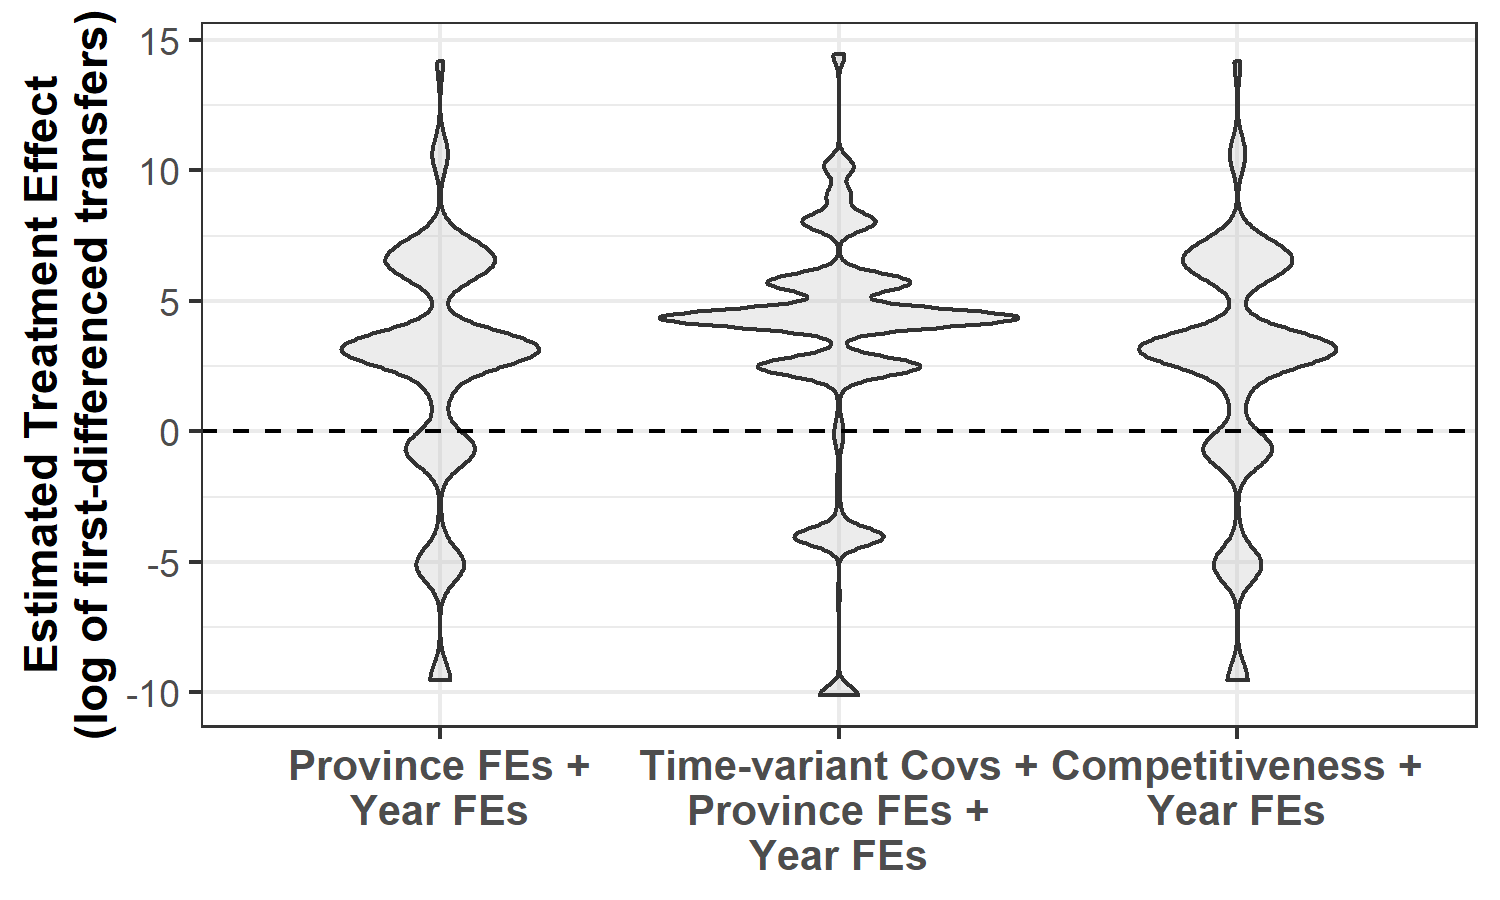
\includegraphics[]{figure/210202_impute_results_2011.png}
	\captionsetup{singlelinecheck=off}
	\caption[Estimated linear fixed effects treatment effects using simulated vote shares]{Distribution of estimates of instantaneous treatment effects on log of first-differenced central transfers using linear fixed effects models on simulated samples. Each sample may include a different set of central candidate defeats and victories.}
	\label{fig:impute_results_2011}
\end{figure}

Distributions of estimated treatment effects using all the linear fixed effects models in the main analysis, obtained from $10000$ independent simulations of the vote shares, are shown in \autoref{fig:impute_results_2011}. It shows that the majority of the estimates are positive. Depending on specification, between 73 to 85\% of the estimates are larger than zero. The distribution of persistent effects are even more reassuring, with 87\% of the estimates being larger than zero across all specifications. In other words, for the true estimate of localized defeats' treatment effects to be negative, the true vote shares of defeated candidates must have taken values that are highly improbable given the winning candidates' performance. Additionally, the estimates in \autoref{fig:lfe_placebo_2011} are close to the minimum values from the distributions, suggesting that almost any feasible allocations of defeated candidates' vote shares can lead to higher treatment effects. Altogether, although this evidence does not eliminate the possibility that the true treatment effect may be negative or close to zero, it does confirm that a ``naive'' approach applying linear fixed effects models to the entire sample of defeated central candidates is likely to be inaccurate. The generalized synthetic control method \citep{Xu2017gsynth}, on the other hand, not only addresses concerns about dynamic causality but also produces estimates that seem much more probable. 

Overall, the positive effect from this analysis suggests that the CPV also reacted to localized defeats of its central candidates in the 2011 election by increasing central transfers to provinces that experienced such defeats. This finding, although much more tentative, is consistent with the result for the 2016 election.
 
\subsection{Responses to localized defeats in the 2007 election}

The analysis for the 2007 election faces even more severe problems than the 2011 analysis. \autoref{fig:lfe_placebo_2007} presents estimates of the persistent treatment effects, along with two sets of placebo treatment effects estimated for 2005 and 2006 (no placebo analysis is done for 2004 due to insufficient data). All these estimates are based on a sample with the entire set of central candidate defeats. The main treatment effects are estimated to be close to zero and not statistically significant, but the large placebo treatment effects suggest that these estimates are likely to be inaccurate. A similar placebo analysis for the instantaneous treatment effects produce nearly identical results.

\begin{figure}[!htbp]
	\centering
	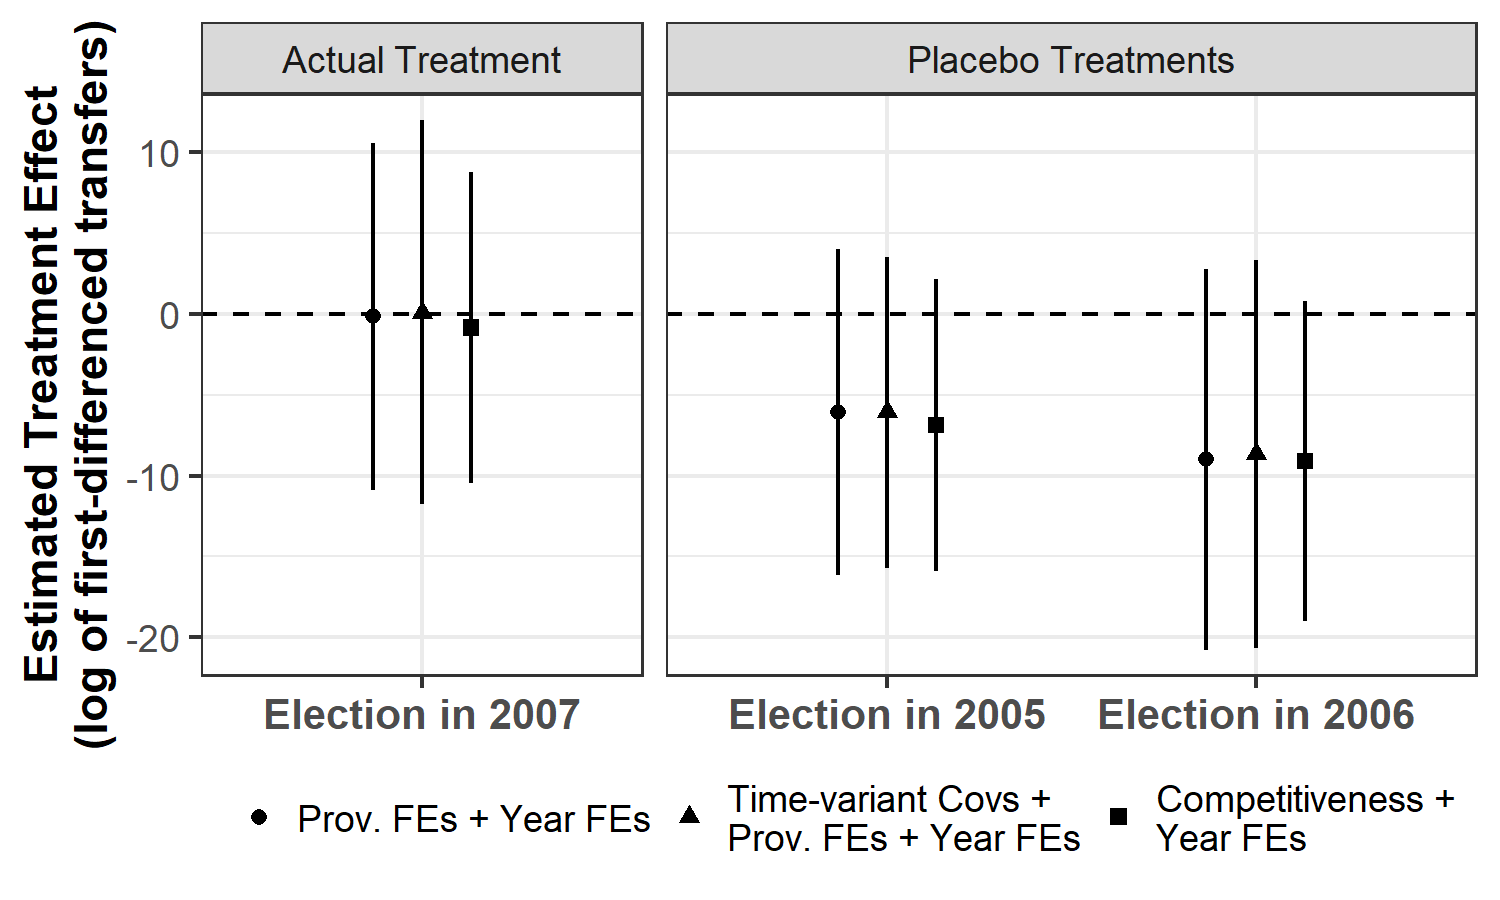
\includegraphics[]{figure/210202_lfe_placebo_2007.png}
	\captionsetup{singlelinecheck=off}
	\caption[Estimated placebo linear fixed effects treatment effects]{Estimates of persistent treatment effects on log of first-differenced central transfers using linear fixed effects models. All central candidate defeats are included in the sample. Error bars show 95\% confidence intervals.}
	\label{fig:lfe_placebo_2007}
\end{figure}

Unlike in the 2011 analysis, the generalized synthetic control method \citep{Xu2017gsynth} is not applicable for 2007 data because there are too few pre-treatment years to construct reliable synthetic controls. There is thus no reliable means to mitigate or eliminate the threat of dynamic causality that is evident in the large placebo effects. 

\begin{figure}[!htbp]
	\centering
	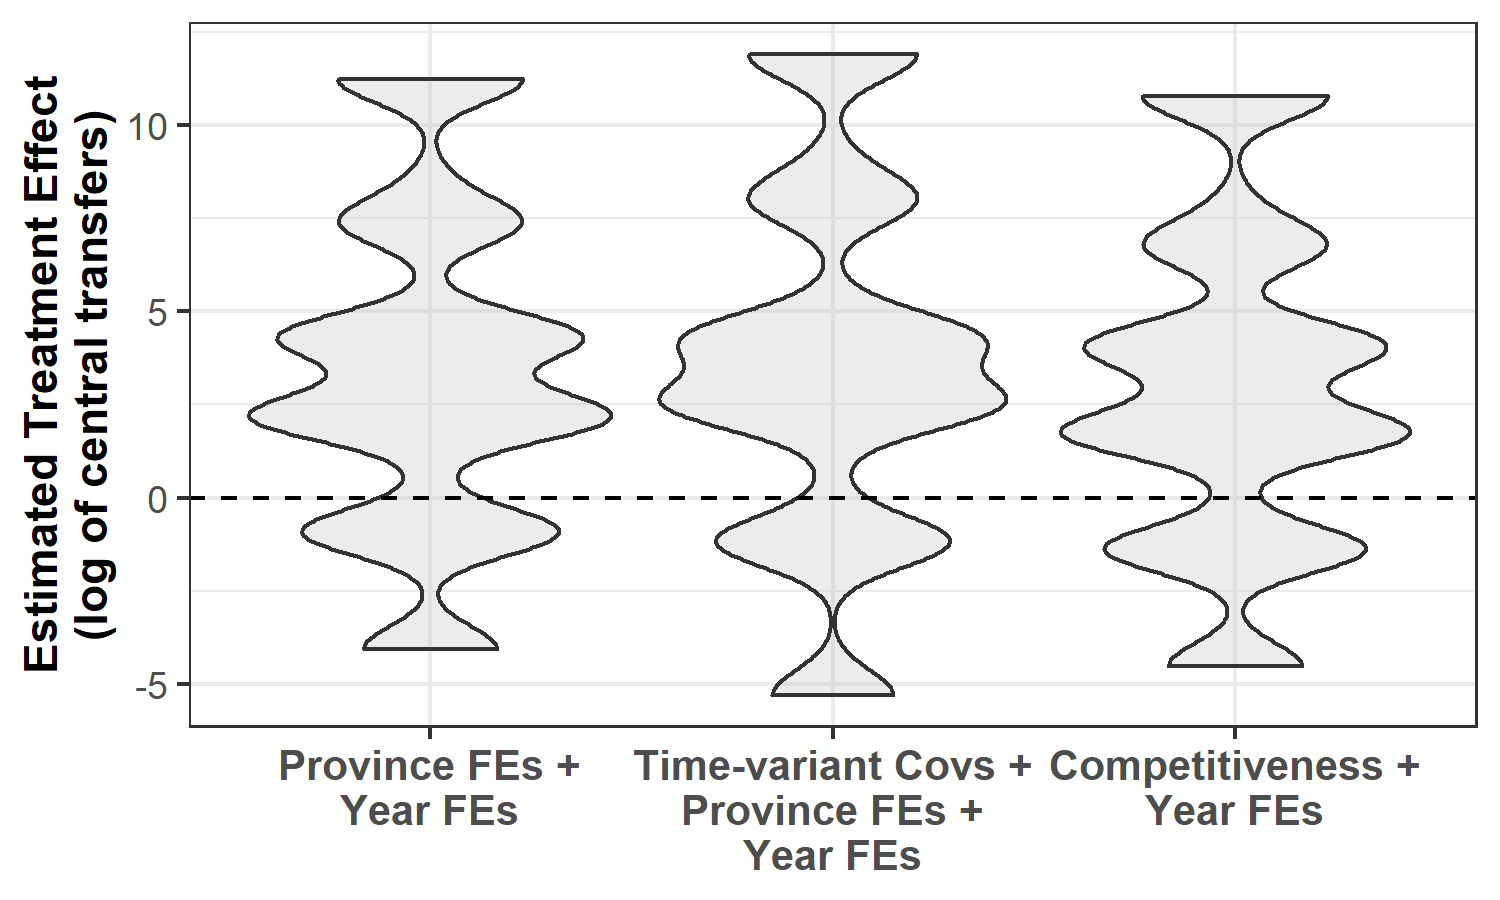
\includegraphics[]{figure/210202_impute_results_2007.png}
	\captionsetup{singlelinecheck=off}
	\caption[Estimated linear fixed effects treatment effects using simulated vote shares]{Distribution of estimates of instantaneous treatment effects on log of first-differenced central transfers using linear fixed effects models on simulated samples. Each sample may include a different set of central candidate defeats and victories.}
	\label{fig:impute_results_2007}
\end{figure}

However, by simulating feasible vote shares of defeated candidates, I still find that the true estimates for the effect of localized defeats on central transfers, obtained when cases of heavy and unsurprising defeats have been excluded, are more likely to be positive. Specifically, \autoref{fig:impute_results_2007}, which shows the distribution of treatment effect estimates obtained from $10000$ simulations of vote shares for the defeated candidates, confirms that the majority of feasible treatment effects are positive. Similar to the 2011 results, both the mean and median of the estimates are positive, with around 84\% of the estimates for the instantaneous treatment effect and between 55 to 73\% of the estimates for the persistent treatment effect found to be larger than zero. Even though much more data is needed for a stronger conclusion, this evidence does offer a reason to believe that the true treatment effects are larger than those found by the ``naive'' linear fixed effects models. Indeed, they are much more likely to be positive, which is consistent with the results for both the 2011 and 2016 elections.

\clearpage

\section{Causal mechanism: development and administrative spending}
\label{app:mechanisms}

In the main manuscript, I argue that a narrative in which the CPV increased central transfers to provinces in which it suffered defeats to placate dissatisfied voters must be accompanied by evidence of an increase in development spending and an absence of cuts in administrative spending. Table \ref{tab:lfe_mech} and Figure \ref{fig:synth_rdd_mech} present this evidence, with the former presenting estimates from linear fixed effects model and the latter showing graphically the results from the local randomization regression discontinuity and generalized synthetic control analyses. As evident, the treatment effect on development spending is positive and statistically significant across all three analyses. The bottom panels of Figure \ref{fig:synth_rdd_mech} also suggest that the effect on development spending is stable over time. Estimates for the treatment effect on administrative spending are found to be statistically significant (at the .1 level) only in the local randomization regression discontinuity analysis and are small in magnitude. The last three columns of Table \ref{tab:lfe_mech} show that the effect on administrative spending are nearly zero, and consistently trending towards being positive across all specifications. Altogether, the three different analyses confirm that development spending increased following central candidate defeats and that administrative spending has remained the same or even increased by a small amount.

Compared to the analyses in the main manuscript, the only difference is that the linear fixed effects models in this section do not use log-differenced outcome. This is because detailed budget breakdowns are available only for a subset of provinces, and then they are sporadically missing for some years. Calculating log-differences would only exacerbate this missingness. This caveat changes the interpretation of the treatment effect's magnitude but does not compromise its validity, as every specification still passes all placebo tests.


% Table created by stargazer v.5.2.2 by Marek Hlavac, Harvard University. E-mail: hlavac at fas.harvard.edu
% Date and time: Fri, Feb 12, 2021 - 2:46:47 PM
\begin{table}[!htbp] \centering 
  \caption{Estimated instantaneous treatment effects of localized defeats on log of development and administration expenditures from linear fixed effects models. Cluster-robust standard errors appear in parentheses.} 
  \label{tab:lfe_mech} 
\begin{tabular}{@{\extracolsep{5pt}}lcccccc} 
\\[-1.8ex]\hline 
\hline \\[-1.8ex] 
 & \multicolumn{3}{c}{Development Expenditure} & \multicolumn{3}{c}{Administrative Expenditure} \\ 
\\[-1.8ex] & (1) & (2) & (3) & (4) & (5) & (6)\\ 
\hline \\[-1.8ex] 
 Treatment Effect & 0.445$^{**}$ & 0.456$^{**}$ & 0.340$^{*}$ & 0.071 & 0.072 & 0.054 \\ 
  & (0.223) & (0.219) & (0.205) & (0.067) & (0.069) & (0.063) \\ 
 \hline \\[-1.8ex] 
Election Competitiveness &  &  & Yes &  &  & Yes \\ 
Time-invariant Covariates &  & Yes &  &  & Yes &  \\ 
Province FEs & Yes & Yes &  & Yes & Yes &  \\ 
Year FEs & Yes & Yes & Yes & Yes & Yes & Yes \\ 
\hline \\[-1.8ex] 
N & 66 & 66 & 66 & 66 & 66 & 66 \\ 
R$^{2}$ & 0.871 & 0.877 & 0.544 & 0.805 & 0.805 & 0.597 \\ 
\hline 
\hline \\[-1.8ex] 
\multicolumn{7}{l}{$^{*}$p $<$ .1; $^{**}$p $<$ .05; $^{***}$p $<$ .01} \\ 
\end{tabular} 
\end{table} 


\begin{figure}[!htbp]
	\centering
	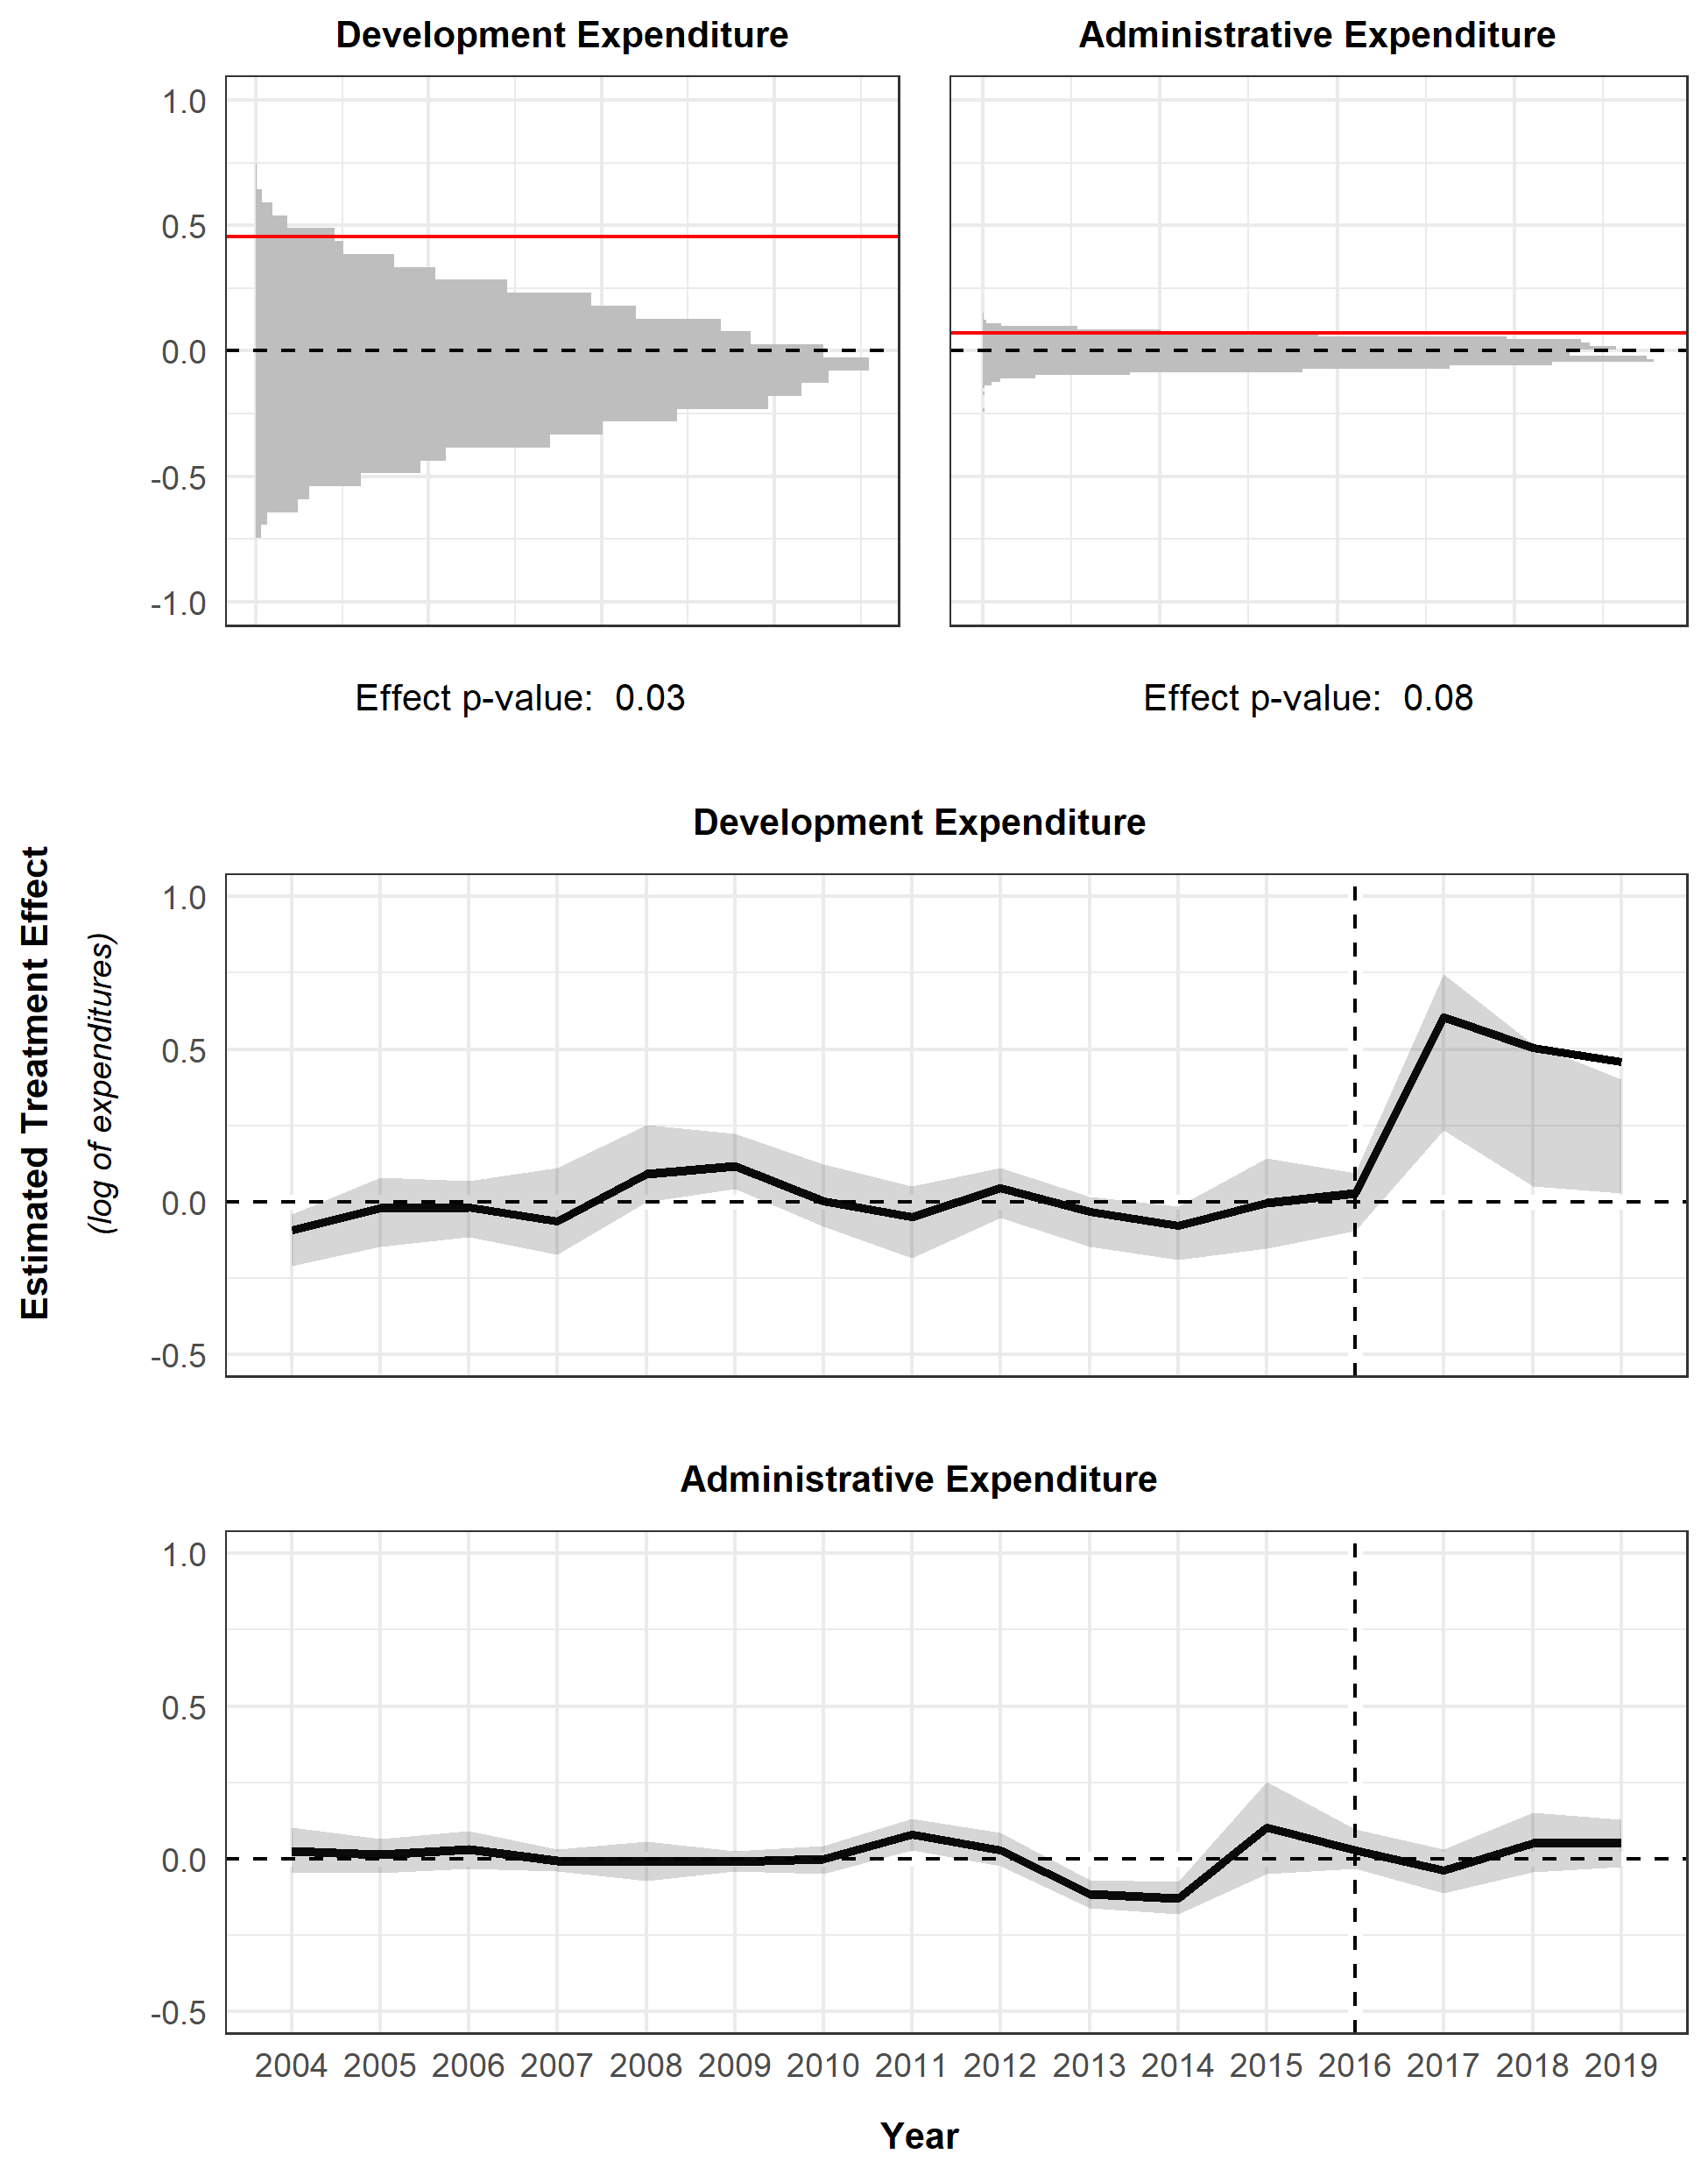
\includegraphics[]{figure/210202_mech_results.png}
	\captionsetup{singlelinecheck=off}
	\caption[Estimated RDD and synthetic control treatment effects]{Estimates of treatment effects on development and administrative expenditure using RDD under the local randomization approach and the generalized synthetic control method. The RDD plots show estimates of instantaneous treatment effects; the generalized synthetic control plots show treatment effects for every year.}
	\label{fig:synth_rdd_mech}
\end{figure}

\clearpage

\section{Individual Accounts of Provinces with Central Candidate Defeats}
\label{app:qualitative}

Excluding Hanoi and Ho Chi Minh City, there are five provinces in which one or more central candidates have suffered defeat in the 2016 election: Can Tho, Dong Thap, Phu Yen, Soc Trang and Tra Vinh. Looking closely into each individual defeat and the post-election dynamic in each province, some patterns clearly emerge. First, it is not straightforward to pinpoint exactly why each central candidate was defeated. Even though most central candidates run against relatively high-ranked (and presumably popular) local competitors, this should not have compromised their chances because the electoral rules allow for multiple seats in each districts. This means that central candidate and the top local candidates do not have to compete against each other as long as they outperform the second or third strongest local candidate. However, in these five provinces, not only did the top local candidates captured more votes than necessary for them to win, but in many cases the remaining votes also went evenly to the local candidates, such that the central candidate ended up with fewer votes than even the weaker local candidates. In some cases the central candidates did not even secure enough vote to cross the 50\% threshold.

Second, even considering the various ways central candidates lost their elections, all five provinces received increases in central transfers, with the 2016 election marking a break point in their funding patterns. In the three provinces for which detailed data is available, 2017 also saw the groundbreaking of several major and highly visible public projects.

Third, in none of these provinces did provincial officials seem to suffer from any form of punishment. Instead, a number of them even secured promotion to higher positions in Hanoi, while the rest were allowed to finish their career in the same position.

In light of these dynamics, it seems very plausible that the central government did choose to uniformly interpret the central candidate defeats in these five provinces as evidence of faltering support and respond with a placation strategy. Even more clearly, the regime has evidently decided to dismiss the possibility that local officials were at fault. Below are the detailed accounts of the central candidate defeats and of the post-election dynamics in all five provinces.

\subsection{Can Tho}

\paragraph{Election Results.} 

In Can Tho's second electoral district, the 2016 election saw four candidates competed for two seats in the VNA. Among them, Nguyen Van Quyen, a 63-year-old native of Ninh Binh, was the central candidate. He was the Party Secretary and Chairman of the Vietnam Lawyers Association--a state-sanctioned organization of legal professionals operating in parallel with the Vietnam Bar Association. Outside of his role in the Lawyers Association, Nguyen Van Quyen also served in the central leadership of Vietnam Fatherland Front (VFF)--the umbrella institution with which all mass organizations must be affiliated--and in a 16-delegate committee on judicial reforms within the CPV central leadership.

Also competing in this district are three local candidates: Tran Quoc Trung, the sitting Party Secretary of Can Tho and member of the CPV Central Committee; Ngo Trung Quan, a local business owner who also held a rank-and-file position in the VFF Central Committee; and Dao Thi Sa Ron, a vice-principal of a local public school. 

\begin{table}[htb]
	\caption{Candidate profiles and election results, Can Tho's second electoral district}
	\label{tab:results_CanTho}
	\resizebox{\textwidth}{!}{%
		\begin{tabular}[t]{@{}llllll@{}}
			\\[-1.8ex] 
			\hline
			\hline
			\\[-1.8ex]
			Name & Age & Gender & Nominator & Professional Profile  & Vote Share (\%) \\ \midrule
			Tran Quoc Trung & 56  & Male   & Local & \begin{tabular}[c]{@{}l@{}}Can Tho Party Secretary\\ Member, \\ \hspace{10pt} CPV Central Committee\end{tabular} & 74.4  \\ \\[-1.8ex] \hline \\[-1.8ex]
			Ngo Trung Quan  & 56  & Male   & Local & \begin{tabular}[c]{@{}l@{}}Member, \\ \hspace{10pt} VFF Central Committee\\ Local Business Owner\end{tabular}    & 49.1   \\ \\[-1.8ex] \hline \\[-1.8ex]
			\textbf{Nguyen Van Quyen} & 63 & Male & Central (VFF) & \begin{tabular}[c]{@{}l@{}} Chairman, \\ \hspace{10pt} Vietnam Lawyers Association\\ Deputy Party Secretary and Vice Chairman, \\ \hspace{10pt} VFF Central Committee\\ Member, \\ \hspace{10pt} CPV Committee on Judicial Reforms\end{tabular} & 47.1 \\ \\[-1.8ex] \hline \\[-1.8ex]
			Dao Thi Sa Ron  & 43  & Female & Local & \begin{tabular}[c]{@{}l@{}} Vice Principal, \\ \hspace{10pt} Can Tho Boarding School for \\ \hspace{10pt} Ethnic Minorities \end{tabular} & 28.2 \\
			\\[-1.8ex] 
			\hline
			\hline
			\\[-1.8ex]
		\end{tabular}%
	}
\end{table}

With two seats up for contest, it would have been possible for both the central candidate Nguyen Van Quyen and the provincial chief Tran Quoc Trung to both win. With each voter casting two votes, the total vote shares among all four candidates in this election would be 200\%. However, because Tran Quoc Trung ended up securing a large number of votes--74.35\%--the remaining vote shares were split thinly among all three remaining candidates, as seen in Table \ref{tab:results_CanTho}. As a result, none of them secured approval from more than 50\% of the voters, thus failing to pass the minimum threshold for election. Nguyen Van Quyen himself was supported by 47.1\% of the voters.

\paragraph{Funding Patterns.} 

Because Tran Quoc Trung was the top provincial chief of Can Tho, and because his large vote shares definitely played a role in Nguyen Van Quyen's defeat, the CPV could interpret the election result in Can Tho either as an evidence of Tran Quoc Trung exerting too much effort to get himself elected, or of Can Tho voters' disapproval of the central regime. An increase in central transfers to Can Tho would show that the CPV believes in the latter interpretation. 

Yet, another hypothesis suggests that increases in transfers to provinces with defeated central candidates could have resulted from these provinces having more local candidates elected and thus a greater voice in the budget allocation process. However, in the case of Can Tho, because no local candidate captured the empty seat,\fnote{In a second election round in which three defeated candidates competed for the empty seats, Nguyen Van Quyen won with 55.11\% of votes and ended up taking this seat.} this election result did not lead to an increased representation for the province in the VNA. An increase in central transfers to Can Tho therefore could not have been triggered by VNA representation. Evidence of this effect still manifesting would thus work against this alternative hypothesis.

There is indeed evidence of an increase in central transfers in \autoref{tab:fund_CanTho}. Since the early 2000s, Can Tho has consistently been a net contributor to the national budget, meaning that it always sends to Hanoi more than it receives back in central transfers. Since 2014, Can Tho's contribution burden has been steadily increasing, reaching the all-time high of 2411 billion VND in 2016. Starting from 2017, however, the burden abruptly embarked on a downward trajectory, dropping for two continuous year before going back up in 2019. This trajectory results in a net decrease in Can Tho's contribution--and hence an increase in how much tax money the province gets to keep--from an average of 1920 billion VND per year in the three pre-election years to an average of 1900 billion VND per year in the three post-election years, despite the economy's steady growth throughout this period.

\begin{table}[]
	\centering
	\caption{Net transfers to Can Tho, 2014-2019. Negative values denote net contribution from Can Tho to the national budget.}
	\label{tab:fund_CanTho}
	\begin{tabular}{@{}lr@{}}
		\toprule
		Year & \multicolumn{1}{c}{Net Transfers (Bil. VND)}  \\ \midrule
		2014 & $-1340$                    \\
		2015 & $-2022$                    \\
		2016 & $-2411$                    \\ \midrule
		2017 & $-2239$                    \\
		2018 & $-1495$                   \\
		2019 & $-1963$                    \\ \bottomrule
	\end{tabular}
\end{table}

A more rigorous way to look at the effect of central candidates on Can Tho's funding pattern is through the individual treatment effect obtained from the generalized synthetic control method. As evident in Figure \ref{fig:synth_mech} that Can Tho did indeed experience increased central transfers between 2017 and 2019 when compared to the synthetic control. Specifically, following a small dip, the Can Tho's net transfers rose to be larger than that of the synthetic control for both subsequent years. Both positive effects are statistically significant, and, counting also the initial dip, average to an increase of about .15 on the log scale. This average increase is also larger than any year-to-year increase ever observed in Can Tho since data becomes available. While this finding is far from conclusive--especially given the statistically significant differences between Can Tho and the synthetic control in some pre-treatment periods--it does offer good evidence that something other than negotiation and bargaining through representation is driving the main treatment effects.

\begin{figure}[!htb]
	\centering
	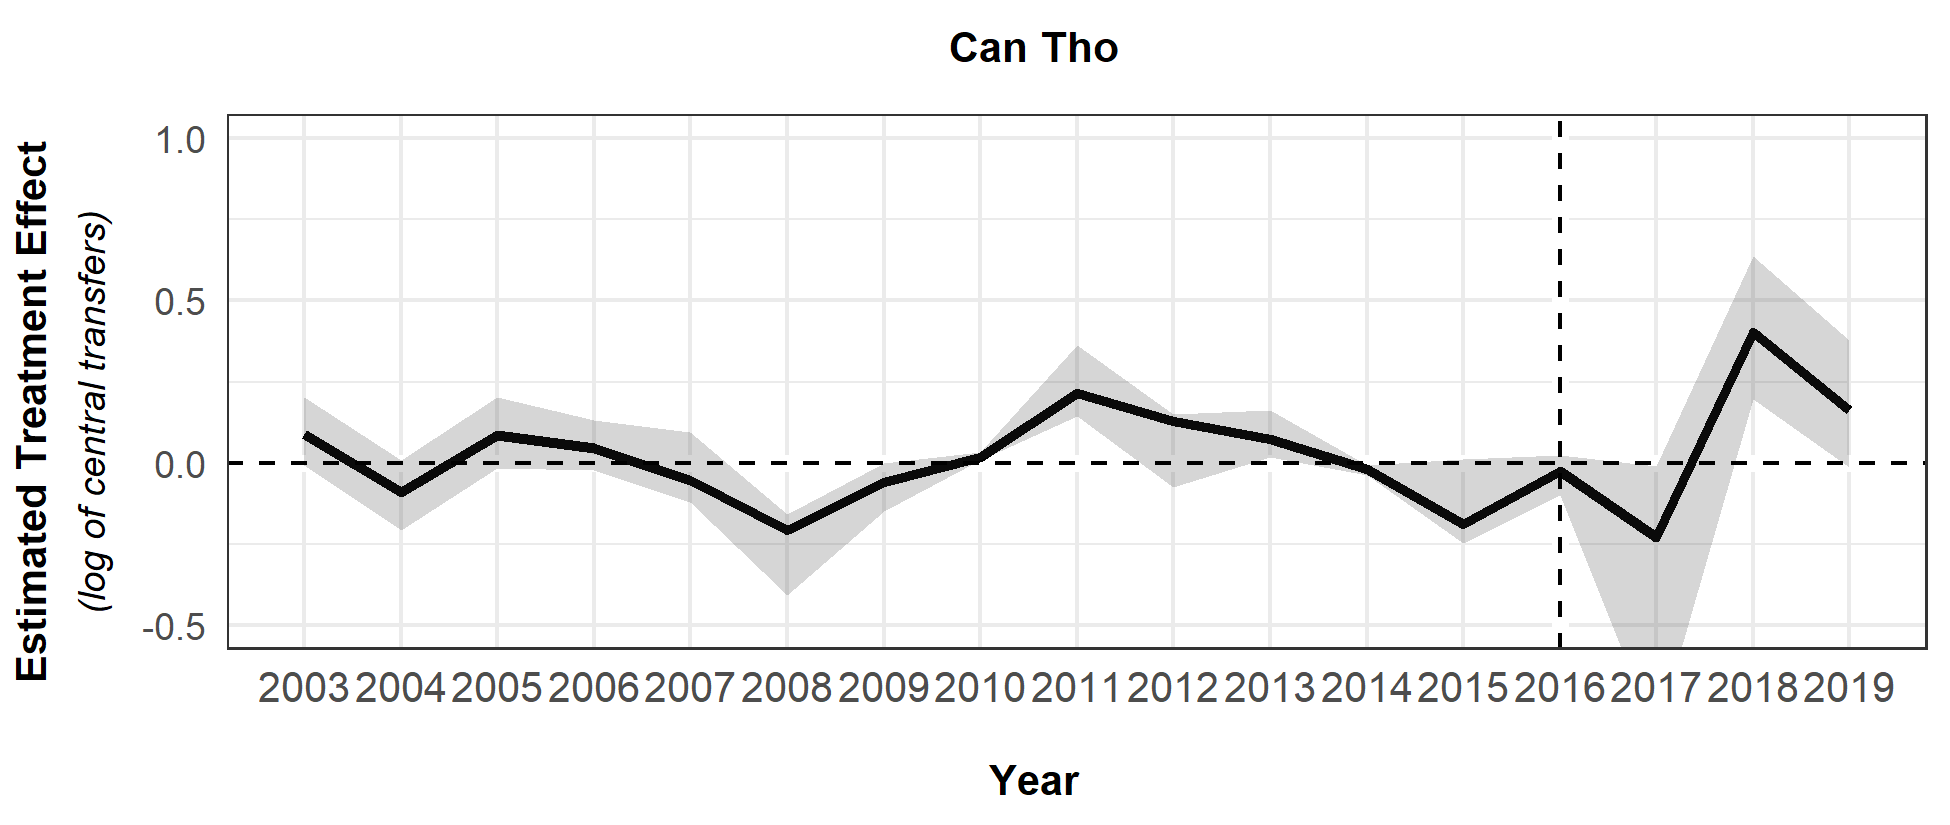
\includegraphics[]{figure/210202_synth_results_CanTho.png}
	\captionsetup{singlelinecheck=off}
	\caption[Individual synthetic control treatment effect]{Individual estimate of treatment effects on central transfers for Can Tho, estimated using the generalized synthetic control method similar to \autoref{fig:synth_placebo}.}
	\label{fig:synth_mech}
\end{figure}

\paragraph{Public Projects.} 

\autoref{tab:projects_CanTho} shows a list of major public projects that begin construction in Can Tho in 2017. It includes a major (500 bed) oncology hospital, a major ring road that would go through the Can Tho airport and connect two highways running through the province, two separate waterway embankment projects, a new clean water system servicing multiple districts, along with other projects targeting existing infrastructure. 

This list of projects were obtained from Can Tho's budget documents for 2017-2020. Because the budget breakdown in these documents is not detailed enough, it is not possible to identify how much each individual project benefited from each increase in central transfers. However, the budget breakdown occasionally shows how much of the budget is expected to come from local, central, or foreign funds, and I exclude all projects that are known to rely completely on local funds. This limits the list to projects that are highly likely to have benefited from central transfers.

\begin{table}[!htb]
	\centering
	\begin{tabular}{@{}llr@{}}
		\\[-1.8ex] 
		\hline
		\hline
		\\[-1.8ex]
		Project Name & Project type & \multicolumn{1}{l}{\begin{tabular}[c]{@{}l@{}}Total Budget \\ (Bil. VND)\end{tabular}} \\ \midrule
		Can Tho Oncology Hospital                 & New construction          & 1727                                           \\		
		Can Tho Airport Ring Road                 & New construction          & 137                                            \\
		Waterway embankment--Ninh Kieu district & New construction          & 315                                            \\
		Waterway embankment--Binh Thuy district & New construction          & 94                                             \\
		Rural clean water system                  & New construction          & 121                                            \\
		Huynh Phan Ho Road                        & Repair/renovation/improvement & 140                                            \\
		Can Tho City Social Protection Center     & Repair/renovation/improvement & 
		50												\\
		Can Tho City Drug Rehabilitation Center   & Repair/renovation/improvement & 16                                             \\
		\\[-1.8ex] 
		\hline
		\hline
		\\[-1.8ex]
	\end{tabular}
	\caption{Major public projects that begin construction in Can Tho in 2017. Total budget includes all sources of funding both domestic and foreign. Projects that are completely funded by the local budget are excluded.}
	\label{tab:projects_CanTho}
\end{table}

\paragraph{Career Trajectories of Provincial Leaders.} 

During the 2016 election, the two top leadership positions in Can Tho were held by Party Secretary Tran Quoc Trung and People's Committee (PCOM) Chairman Vo Thanh Thong. Tran Quoc Trung, who himself ran and won convincingly, stayed in his position for the full duration of his term until September 2020 when he reached the mandated retirement age. Vo Thanh Thong continued to serve in the same position until May 2019 when he was promoted to be the Deputy Minister of Planning and Investment.

\subsection{Dong Thap}

\paragraph{Election Results.} 

The central candidate defeat in Dong Thap happened in the first electoral district, in which the Vice Chairman of the VNA Committee on Laws Nguyen Kim Hong ran against three local candidates. With two seats available and each voter casting two votes, Nguyen Kim Hong would have won even if he had come behind a strong local candidate. Out of three local candidates, two were relatively stronger--Tran Van Cuong, political commissar of the provincial military command, and Huynh Minh Tuan, director of a department-level agency--although neither belonged to the province's top leadership. This absence of a clear front runner was reflected well in the final results. However, even when they secure similar shares of votes, both these local candidates managed to outperform Nguyen Kim Hong. This suggests that a large number of voters have decided to cast both their votes for local candidates. As a result, the district's two seats went to Tran Van Cuong and Huynh Minh Tuan, with Nguyen Kim Hong trailing closely behind.

\begin{table}[!htb]
	\caption{Candidate profiles and election results, Dong Thap's first electoral district}
	\label{tab:results_DongThap}
	\resizebox{\textwidth}{!}{%
		\begin{tabular}[t]{@{}llllll@{}}
			\\[-1.8ex] 
			\hline
			\hline
			\\[-1.8ex]
			Name & Age & Gender & Nominator & Professional Profile  & Vote Share (\%) \\ \midrule
			Tran Van Cuong & 52  & Male   & Local & \begin{tabular}[c]{@{}l@{}}Member, \\ \hspace{10pt} Dong Thap Party Committee \\  Political Commissar, \\ \hspace{10pt} Dong Thap Military Command \end{tabular} & 60.3  \\ \\[-1.8ex] \hline \\[-1.8ex]
			\textbf{Nguyen Kim Hong}  & 57  & Male   & Central (VNA) & \begin{tabular}[c]{@{}l@{}}Vice Chairman, \\ \hspace{10pt} VNA Committee on Laws \end{tabular}    & 48.9   \\ \\[-1.8ex] \hline \\[-1.8ex]
			Nguyen Van Thong & 53 & Male & Local & \begin{tabular}[c]{@{}l@{}} Deputy Head, \\ \hspace{10pt} Tam Nong District Division of Agriculture \\\hspace{10pt} and Rural Development
			 \end{tabular} & 34.1 \\ \\[-1.8ex] \hline \\[-1.8ex]
			Huynh Minh Tuan  & 36  & Male & Local & \begin{tabular}[c]{@{}l@{}}Member, \\ \hspace{10pt} Dong Thap Party Committee \\ Director, \\ \hspace{10pt} 
				Dong Thap Department of Science and  \\\hspace{10pt} Technology \end{tabular} & 56.3 \\
			\\[-1.8ex] 
			\hline
			\hline
			\\[-1.8ex]
		\end{tabular}%
	}
\end{table}

\paragraph{Funding Patterns.} 

Compared to the case of Can Tho, the election result in Dong Thap resembles more closely the narrative of voters expressing dissatisfaction with the regime by voting against its favored candidates. The post-election shift in central transfers to Dong Thap seems to suggest that the CPV shares this view. Specifically, in 2017 Dong Thap saw an unprecedented increase in central transfers of 1153 billion VND, bringing net transfers to an all-time high of 2683 billion VND. Central transfers to Dong Thap continued to increase in the following year, bringing the three-year average from 2017 to 2019 to 2,980 billion VND per year, almost 60\% higher than the average of 1,870 billion VND per year in the 2014-2016 period.

\begin{table}[!htb]
	\centering
	\caption{Net transfers to Dong Thap, 2014-2019.}
	\label{tab:fund_DongThap}
	\begin{tabular}{@{}lr@{}}
		\toprule
		Year & \multicolumn{1}{c}{Net Transfers (Bil. VND)}  \\ \midrule
		2014 & $1821$                    \\
		2015 & $2261$                    \\
		2016 & $1530$                    \\ \midrule
		2017 & $2683$                    \\
		2018 & $2992$                   \\
		2019 & $3246$                    \\ \bottomrule
	\end{tabular}
\end{table}
%\begin{figure}[!htb]
%	\centering
%	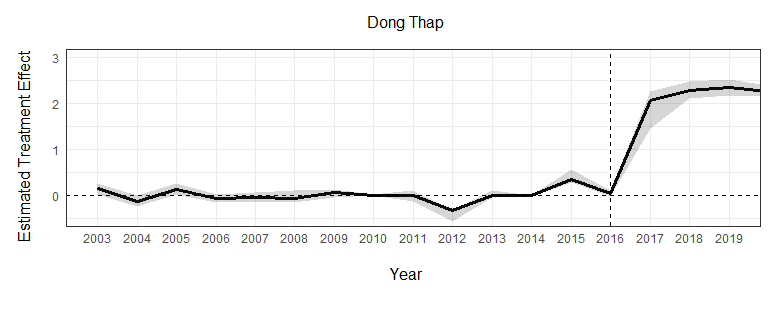
\includegraphics[width=\textwidth]{figure/200916_synth_results_DongThap.png}
%	\captionsetup{singlelinecheck=off}
%	\caption[Individual synthetic control treatment effect]{Individual estimate of treatment effects on central transfers for Dong Thap, estimated using the generalized synthetic control method similar to \autoref{fig:synth_placebo}.}
%	\label{fig:synth_dongthap}
%\end{figure}
\paragraph{Public Projects.} Dong Thap's annual budget documents do not contain a detailed list of public projects in the province. However, other legal documents, for example the appendix of the Decision 110/2017/NQ-HDND issued by the Dong Thap People's Council, do provide information on some public projects being proposed and approved within 2017. These documents show that in 2017 alone Dong Thap had an impressive portfolio of projects that were recently approved for construction, including two industrial zones, three daycare centers, two kindergartens, nine primary schools, five junior secondary schools, a bridge, and two road expansions. Although it is not clear how many of these projects actually begun construction and if so when (as opposed to being delayed or canceled), this list alone offers strong evidence of a burst of public project construction in 2017.

\paragraph{Career Trajectories of Provincial Leaders.} The two provincial leaders in Dong Thap during the 2016 election were Party Secretary Le Minh Hoan and PCOM Chairman Nguyen Van Duong. Following the election, both officials remained in their position until the end of their terms in 2020. Le Minh Hoan was then promoted to be the Deputy Minister of Agriculture and Rural Development in October 2020, and Nguyen Van Duong retired in December 2020 upon reaching the mandatory retirement age. Neither received any form of punishment.

\subsection{Phu Yen}

\paragraph{Election Results.} 

In Phu Yen's first electoral district, five candidates contested for three available seats. One of the seats was expected to go to the central candidate Y Thong, a native of Phu Yen who was serving as a standing member of the VNA's Council for Ethnic Minority Affairs, a VNA oversight body tasked with governing of the Government's activities that are related to ethnic minority affairs. The two remaining seats were expected to go to Nguyen Thai Hoc, a senior member within Phu Yen's party organization and a committee member in the VNA, and Phan Anh Khoa, the political commissar of Phu Yen military command. On election day, however, an unexpectedly strong performance by Pham Thi Minh Hien, deputy director of Phu Yen's Department of Labour, War Invalids and Social Affairs, allowed her to finish just ahead of Y Thong.

It is unclear why more votes went to Pham Thi Minh Hien, a young official with a relatively low profile, instead of the central candidate Y Thong. It should be noted, however, that both Y Thong and Ma Thanh, the other defeated candidate in this election, were members of the Ede ethnic group. Even though Phu Yen is home to a large Ede population, this ethnic group still comprises less than 5\% of the local population. As member of the VNA Council for Ethnic Minority Affairs, Y Thong may have been associated with the regime's efforts to enhance the visibility of minority groups. The votes against Y Thong may have reflected the Kinh majority's aversion to these efforts.

\begin{table}[htb]
	\caption{Candidate profiles and election results, Phu Yen's first electoral district}
	\label{tab:results_PhuYen}
	\resizebox{\textwidth}{!}{%
		\begin{tabular}[t]{@{}llllll@{}}
			\\[-1.8ex] 
			\hline
			\hline
			\\[-1.8ex]
			Name & Age & Gender & Nominator & Professional Profile  & Vote Share (\%) \\ \midrule
			Pham Thi Minh Hien & 38  & Female   & Local & \begin{tabular}[c]{@{}l@{}}Deputy Director, \\ \hspace{10pt} Phu Yen Department of Labour, \\ \hspace{10pt} War Invalids and Social Affairs \end{tabular} & 55.0  \\ \\[-1.8ex] \hline \\[-1.8ex]
			Nguyen Thai Hoc  & 44  & Male   & Local & \begin{tabular}[c]{@{}l@{}}Standing Member, \\ \hspace{10pt} Phu Yen Party Committee \\ Member, \\ \hspace{10pt} VNA Judiciary Commisttee \\ Member, \\ \hspace{10pt} Phu Yen Lawyers Association \end{tabular}    & 84.1   \\ \\[-1.8ex] \hline \\[-1.8ex]
			Phan Anh Khoa & 51 & Male & Local & \begin{tabular}[c]{@{}l@{}} Deputy Party Secretary and \\ Political Commissar, \\ \hspace{10pt} Phu Yen Military Command \end{tabular} & 75.4 \\ \\[-1.8ex] \hline \\[-1.8ex]
			\textbf{Y Thong } & 50  & Male & Central (VNA) & \begin{tabular}[c]{@{}l@{}}Standing Member, \\ \hspace{10pt} VNA Committee for Ethnic\\ \hspace{10pt} Minority Affairs \end{tabular} & 49.9 \\ \\[-1.8ex] \hline \\[-1.8ex]
			Ma Thanh  & 48  & Male & Local & \begin{tabular}[c]{@{}l@{}}Member, \\ \hspace{10pt} Phu Yen Party Committee \\ Party Secretary, \\ \hspace{10pt} Song Hinh District Party Committee  \end{tabular} & 31.0 \\ 
			\\[-1.8ex] 
			\hline
			\hline
			\\[-1.8ex]
		\end{tabular}%
	}
\end{table}

\paragraph{Funding Patterns.} 

Even though the true cause behind Y Thong's defeat may never be known, the CPV clearly decided to increase the level of central transfers to Phu Yen. Prior to the 2016 election, Phu Yen has experienced a downward trajectory in net transfers, which the level of transfers falling from 2100 billion VND in 2014 to 1750 billion VND in 2016. In 2017, however, the province saw an unprecedented increase of more than 900 billion VND, bringing the level of net transfers to a record 2600 billion VND.

\begin{table}[]
	\centering
	\caption{Net transfers to Phu Yen, 2014-2019.}
	\label{tab:fund_PhuYen}
	\begin{tabular}{@{}lr@{}}
		\toprule
		Year & \multicolumn{1}{c}{Net Transfers (Bil. VND)}  \\ \midrule
		2014 & $2104$                    \\
		2015 & $1966$                    \\
		2016 & $1741$                    \\ \midrule
		2017 & $2644$                    \\
		2018 & $2807$                   \\
		2019 & $2735$                    \\ \bottomrule
	\end{tabular}
\end{table}

%\begin{figure}[!htb]
%	\centering
%	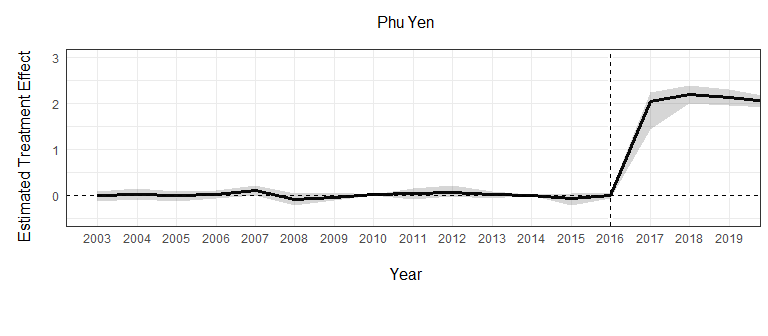
\includegraphics[width=\textwidth]{figure/200916_synth_results_PhuYen.png}
%	\captionsetup{singlelinecheck=off}
%	\caption[Individual synthetic control treatment effect]{Individual estimate of treatment effects on central transfers for Phu Yen, estimated using the generalized synthetic control method similar to \autoref{fig:synth_placebo}.}
%	\label{fig:synth_phuyen}
%\end{figure}


\paragraph{Public Projects.} Information about public project construction in Phu Yen is not available. However, it is publicly known that the province began construction of a large public park on the beach front of Tuy Hoa city (the primary municipality of the province), as well as a junior secondary school in Dong Hoa district.

\paragraph{Career Trajectories of Provincial Leaders.} 

Despite their possible role in a central candidate defeat, both provincial leaders in Phu Yen during the 2016 election received promotion at the end of their term. Specifically, Party Secretary Huynh Tan Viet was promoted to head the Party Committee of Central-level Agencies, the umbrella party organization to which every party organization within government agencies at the central level must report. PCOM Chairman Hoang Van Tra, who also ran and won in the 2016 VNA election, was promoted to Deputy Chairman of the Central Inspection Commission, the party organization directly in charge of the anti-corruption campaign that would unfold soon after the election.

\subsection{Tra Vinh}

\paragraph{Election Results.} 

In Tra Vinh's first electoral district, the central candidate Sa Van Khiem suffered a shocking defeat when he came in last against four local candidates. A member of the VNA Secretariat and director of a department within the Office of the National Assembly, Sa Van Khiem was clearly a high-ranking member in the VNA. In a district with five candidate and three available seats, it would have been possible for him to come in behind two of the province's stronger candidates and still win. Moreover, among the local candidates, only Ngo Chi Cuong, deputy secretary of the provincial party committee, was actively promoted by grassroots cadres. Thus, the fact that Sa Van Khiem received fewer votes than all the local candidates, including two who only served as deputy directors of department-level agencies, was extremely unexpected. The large number of votes--78.1\%--for Ngo Chi Cuong could have contributed to Sa Van Khiem's defeat, but it was also important that many votes were also spread evenly among the three other local candidates. The latter in particular may have indicated that the votes were cast specifically \textit{against} Sa Van Khiem but not \textit{for} any local candidate.

\begin{table}[htb]
	\caption{Candidate profiles and election results, Tra Vinh's first electoral district}
	\label{tab:results_TraVinh}
	\resizebox{\textwidth}{!}{%
		\begin{tabular}[t]{@{}llllll@{}}
			\\[-1.8ex] 
			\hline
			\hline
			\\[-1.8ex]
			Name & Age & Gender & Nominator & Professional Profile  & Vote Share (\%) \\ \midrule
			Le Van Hong Anh & 47  & Male   & Local & \begin{tabular}[c]{@{}l@{}}Party Secretary and Deputy Director, \\ \hspace{10pt} Phu Yen Department of Science and \\ \hspace{10pt} Technology \end{tabular} & 56.6  \\ \\[-1.8ex] \hline \\[-1.8ex]
			Thach Phuoc Binh  & 38  & Male   & Local & \begin{tabular}[c]{@{}l@{}}Deputy Head, \\ \hspace{10pt}Tra Vinh Party Committee Propaganda \\ \hspace{10pt}Board \end{tabular}    & 58.1   \\ \\[-1.8ex] \hline \\[-1.8ex]
			Ngo Chi Cuong & 49 & Male & Local & \begin{tabular}[c]{@{}l@{}} Standing Deputy Party Secretary, \\ \hspace{10pt} Tra Vinh Party Committee \end{tabular} & 78.1 \\ \\[-1.8ex] \hline \\[-1.8ex]
			\textbf{Sa Van Khiem} & 52  & Male & Central (VNA) & \begin{tabular}[c]{@{}l@{}} Member, \\ \hspace{10pt} VNA Secretariat \\ Director,\\ \hspace{10pt} Department of Ethnic Minority Affairs, \\ \hspace{10pt} Office of the VNA \end{tabular} & 48.3 \\ \\[-1.8ex] \hline \\[-1.8ex]
			Tang Thi Ngoc Mai  & 48  & Female & Local & \begin{tabular}[c]{@{}l@{}}Deputy Director, \\ \hspace{10pt} Tra Vinh Department of Education and \\ \hspace{10pt} Training \end{tabular} & 56.8 \\ 
			\\[-1.8ex] 
			\hline
			\hline
			\\[-1.8ex]
		\end{tabular}%
	}
\end{table}

\paragraph{Funding Patterns.} 

The pattern of central transfers to Tra Vinh also reflects very clearly an increase in the post-election years. Whereas between 2014 and 2016 Tra Vinh had been receiving a steady level of net transfers averaging 2,560 billion VND per year, in 2017 it saw a large increase of 920 billion VND. The increase in transfers persist over the following years, bringing the level of net transfers to Tra Vinh to an average of 3410 billion VND between 2017 and 2019.

\begin{table}[]
	\centering
	\caption{Net transfers to Tra Vinh, 2014-2019.}
	\label{tab:fund_TraVinh}
	\begin{tabular}{@{}lr@{}}
		\toprule
		Year & \multicolumn{1}{c}{Net Transfers (Bil. VND)}  \\ \midrule
		2014 & $2670$                    \\
		2015 & $2553$                    \\
		2016 & $2476$                    \\ \midrule
		2017 & $3395$                    \\
		2018 & $3397$                   \\
		2019 & $3439$                    \\ \bottomrule
	\end{tabular}
\end{table}

%\begin{figure}[!htb]
%	\centering
%	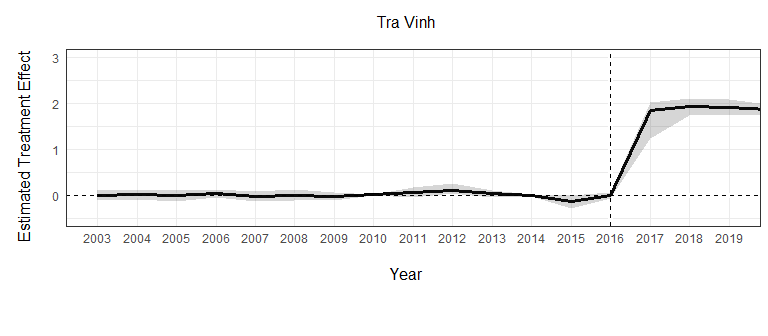
\includegraphics[width=\textwidth]{figure/200916_synth_results_TraVinh.png}
%	\captionsetup{singlelinecheck=off}
%	\caption[Individual synthetic control treatment effect]{Individual estimate of treatment effects on central transfers for Tra Vinh, estimated using the generalized synthetic control method similar to \autoref{fig:synth_placebo}.}
%	\label{fig:synth_TraVinh}
%\end{figure}

\paragraph{Public Projects.} \autoref{tab:projects_TraVinh} shows a list of major public projects in Tra Vinh that began construction in 2017 and did not rely completely on local funds (and thus are more likely to have benefited from increases in central transfers). The list includes a major general hospital of 700 beds, the establishment of basic infrastructure for an agriculture zone, major improvements to the province's connected waterways, and the construction of solid walls for rural kindergartens across the province, as well as a digital database of land use information. 

\begin{table}[!htb]
	\centering
	\caption{Major public projects that begin construction in Tra Vinh in 2017. Total budget includes all sources of funding both domestic and foreign. Projects that are completely funded by local budgets are excluded.}
	\label{tab:projects_TraVinh}
	\begin{tabular}{@{}llr@{}}
		\\[-1.8ex] 
		\hline
		\hline
		\\[-1.8ex]
		Project Name & Project type & \multicolumn{1}{l}{\begin{tabular}[c]{@{}l@{}}Total Budget \\ (Billion VND)\end{tabular}} \\ \midrule
		Tra Vinh General Hospital    & New construction              & 1600 \\
		Agriculture infrastructure   & New construction              & 460  \\
		Waterway dredging            & Repair/renovation/improvement & 379  \\
		Waterway expansion           & Repair/renovation/improvement & 229  \\ 	
		Renovations of kindergartens & Repair/renovation/improvement & 137  \\
		Provincial land use database & Digital                       & 65   \\
		\\[-1.8ex] 
		\hline
		\hline
		\\[-1.8ex]
	\end{tabular}
	
\end{table}

\paragraph{Career Trajectories of Provincial Leaders.} 

Both of Tra Vinh's leaders during the 2016 election--Party Secretary Tran Tri Dung and PCOM Chairman Dong Van Lam--were serving their last terms in office. Tran Tri Dung retired in October 2020 and was succeeded by Ngo Chi Cuong, the very candidate who received the most votes in the first electoral district. Dong Van Lam retired in November 2020.

\subsection{Soc Trang}

\paragraph{Election Results.} 

In Soc Trang's second electoral district, a central defeat happened to Pham Thanh Nam, a department director in the Office of the CPV Central Committee (the administrative and management body of the CPV Central Committee). With the possible exception of Ho Thi Cam Dao who was a standing member of the provincial party committee, the local candidates also running in this election had much weaker profiles compared to Pham Thanh Nam, which should have allowed the latter to easily secure one of the district's three seats. However, because Ho Thi Cam Dao received a very large number of votes--75\%--the remaining votes were split thinly among the remaining candidates, leaving no one with enough votes to clear the 50\% threshold. Pham Thanh Nam secured only 35.9\% of the vote, trailing behind Tran Khac Tam, a local business owner with no formal position in the government.

\begin{table}[htb]
	\caption{Candidate profiles and election results, Soc Trang's second electoral district}
	\label{tab:results_SocTrang}
	\resizebox{\textwidth}{!}{%
		\begin{tabular}[t]{@{}llllll@{}}
			\\[-1.8ex] 
			\hline
			\hline
			\\[-1.8ex]
			Name & Age & Gender & Nominator & Professional Profile  & Vote Share (\%) \\ \midrule
			Ho Thi Cam Dao & 44  & Female   & Local & \begin{tabular}[c]{@{}l@{}}Standing Member, \\ \hspace{10pt} Phu Yen Party Committee \\ Head, \\ \hspace{10pt} Phu Yen Party Committee Mass \\ \hspace{10pt} Mobilization Board \end{tabular} & 75.0  \\ \\[-1.8ex] \hline \\[-1.8ex]
			\textbf{Pham Thanh Nam}  & 52  & Male   & Central (VNA) & \begin{tabular}[c]{@{}l@{}}Member, \\ \hspace{10pt}Inspection Committee \\ \hspace{10pt} Office of the CPV Central Committee  \\ Director, \\ \hspace{10pt} General Department \\ \hspace{10pt} Office of the CPV Central Committee \end{tabular}    & 35.9   \\ \\[-1.8ex] \hline \\[-1.8ex]
			Huynh Lan Phuong & 38 & Female & Local & \begin{tabular}[c]{@{}l@{}} Department Chief, \\ \hspace{10pt} Soc Trang General Hospital \end{tabular} & 20.6 \\ \\[-1.8ex] \hline \\[-1.8ex]
			Tran Khac Tam & 44  & Male & Local & \begin{tabular}[c]{@{}l@{}} Local Business Owner \end{tabular} & 46.8 \\ \\[-1.8ex] \hline \\[-1.8ex]
			Ho Van Thao  & 36  & Male & Local & \begin{tabular}[c]{@{}l@{}} Deputy Director, \\ \hspace{10pt} Center for Applications of Scientific \\ \hspace{10pt}  and Technological Advancements \\ \hspace{10pt} Soc Trang Department of Science and \\ \hspace{10pt} Technology \end{tabular} & 21.4 \\ 
			\\[-1.8ex] 
			\hline
			\hline
			\\[-1.8ex]
		\end{tabular}%
	}
\end{table}

\paragraph{Funding Patterns.} 

Because of the large margin by which Pham Thanh Nam lost his election, Soc Trang was not included in the primary analysis in the main manuscript. However, the post-election shift in net transfers here still closely mirrors the patterns in other provinces. Specifically, whereas Soc Trang had been receiving a steady flow of net transfers averaging 3405 billion VND per year between 2014 and 2016, in 2017 central transfers to this province started to increase rapidly, reaching a high of 5341 billion VND in 2019. The average level of annual transfers for the post-election years from 2017 to 2019 was 4051 billion VND, nearly 20\% higher than that for the pre-election years.

\begin{table}[!htb]
	\centering
	\caption{Net transfers to Soc Trang, 2014-2019.}
	\label{tab:fund_SocTrang}
	\begin{tabular}{@{}lr@{}}
		\toprule
		Year & \multicolumn{1}{c}{Net Transfers (Bil. VND)}  \\ \midrule
		2014 & $3316$                    \\
		2015 & $3510$                    \\
		2016 & $3390$                    \\ \midrule
		2017 & $3460$                    \\
		2018 & $3710$                   \\
		2019 & $4982$                    \\ \bottomrule
	\end{tabular}
\end{table}

\paragraph{Public Projects.} 

Soc Trang's budget documents show that in 2017 the province embarked on several new infrastructure projects. Most notable of those is the construction of an 25.6 kilometer (16 miles) arterial road that would connect Soc Trang City with the new agriculture zone in the southern end of the province. The city also began working on improving Soc Trang City's urban infrastructure, and expanding a major road. Finally, two small hospitals with 100 each were constructed in the districts of Chau Thanh and Cu Lao Dung.

\begin{table}[!htb]
	\centering
	\caption{Major public projects that begin construction in Soc Trang in 2017. Total budget includes all sources of funding both domestic and foreign. Projects that are completely funded by local budgets are excluded.}
	\label{tab:projects_SocTrang}
	\begin{tabular}{@{}llr@{}}
		\\[-1.8ex] 
		\hline
		\hline
		\\[-1.8ex]
		Project Name & Project type & \multicolumn{1}{l}{\begin{tabular}[c]{@{}l@{}}Total Budget \\ (Billion VND)\end{tabular}} \\ \midrule
		Arterial road from Soc Trang City   & New construction              & 1200 \\
		Soc Trang City urban infrastructure & Repair/renovation/improvement & 1057 \\
		Le Hong Phong Road                  & Repair/renovation/improvement & 207  \\
		Chau Thanh General Hospital         & New construction              & 92   \\
		Cu Lao Dung General Hospital        & New construction              & 87   \\ 
		\\[-1.8ex] 
		\hline
		\hline
		\\[-1.8ex]
	\end{tabular}
\end{table}

\paragraph{Career Trajectories of Provincial Leaders.} 

The two leaders heading the Soc Trang provincial governments during the 2016 election was Party Secretary Nguyen Van The and PCOM Chairman Nguyen Van Hieu. Formerly Deputy Minister of Transport before being appointed to Soc Trang in October 2015--presumably to serve a rotation before getting promoted further--Nguyen Van The only had to wait until October 2017 before returning to Hanoi as Minister of Transport, a position he still holds today. Having also run and won a VNA seat in 2016, he also served as the head of the Soc Trang delegate before his promotion. Nguyen Van Hieu was also promoted very shortly after the election to be the Deputy Chair of the Steering Committee for the Southwest. He retired early in October 2017, but only because the CPV abolished the institution of regional steering committees altogether in a major restructuring of the party organization.


\clearpage
\section{Absence of other forms of punishment}
\label{app:punishment}

An alternative hypothesis is that the CPV sees the VNA election results as providing information on both the distribution of regime popularity and the quality of local officials but uses central transfers to react to unhappy citizens, while reserving another form of punishment for incompetent or disloyal provincial officials. More specifically, this hypothesis would require that officials in provinces with central candidate defeats would be fired, demoted, or at least would have their career advancement slowed down following the election.

Although this hypothesis may have held in other in other nondemocratic regimes such as Russia \citep{Myagkov2009}, the specific context of Vietnam makes it less likely. Specifically, Vietnam's leaders rely on punishment much more sparingly, reserving demotion or firing only to very serious transgressions, presumably to maintain a notion of unity among the leadership and preserve confidence in the regime.\fnote{Two illustrative anecdotes suggest that the CPV avoids punishment because it draws attention to disunity within the party, and that it only punishes top officials in case of extreme transgressions. In 2012, when the CPV's highest leadership debated and decided against officially censuring then-PM Nguyen Tan Dung for economic mismanagement, official statements from the Party refers to him only as ``one comrade'' without mentioning any name \citep{voa2012}. Later, in 2017, when the Party's leaders finally decided to punish Ho Chi Minh City's Party Secretary Dinh La Thang and to publicly acknowledge this decision, it was only after mismanagement of PetroVietnam, Vietnam's largest SOE and where Thang had served as chairman between 2009 and 2001, has been found to cost the country close to 150 million USD \citep{BBC2017}.} Logistically, each punishment decision must be preceded by a lengthy formal process: the official in question must first be investigated and found guilty of some serious transgression, then the punishment must be recommended by the disciplinary agency, and finally it must be approved by the larger party apparatus. Depending on the official's seniority, this may require several high-profile votes by members of the Politburo and then by the CPV Central Committee, which always attract public attention.

In addition, in terms of delaying promotion, the CPV only makes major promotion decisions around the time of its Party Congress, which takes place every five year and usually just before an election (presumably so that the election could ratify and legitimize newly appointed leaders). This makes the time lag between one election's outcomes and the next batch of promotion decisions too large for the latter to be useful as punishment for the former.

It is also unlikely that the CPV would be able to issue punishment to officials below provincial officials. The accountability chain in Vietnam follows a pattern of ``double subordination'' \citep[][pg. 8]{Kerkvliet2004}, in which officials at any level are accountable only to the legislature and party organization at its own level and to the government organization at the level above it. This means that district-level officials can only be punished by province-level officials, and commune-level officials can only be punished by district-level officials. 

More importantly, unlike that between the provinces and the central government, center-periphery conflict is much more muted at lower levels of government. Local governance is centered at the province level, meaning that lower-level officials from the district down to grassroots officials are much more accountable to provincial leaders, mostly due to local officials being geographically bound to the provinces. In practice, this means that provincial governments have greater ability to monitor their subordinates, and in many cases are able to manipulate appointments at local levels to staff family members and close allies to lower-level offices. As a result, they face less difficulty maintaining the accountability of lower-level agents and thus have less need to use election results to find out which agents need to be punished.

For these various reasons, it is unlikely that the CPV would have used major forms of punishment in reaction to central candidate defeats in the VNA elections. Concrete evidence below suggests that the regime has indeed refrained from doing so.

\subsection{Following the 2007 and 2011 elections}

First, for those officials who were governing before and during the 2007 and 2001 elections, I show that central candidate defeats have had no impact on their career prospects. To do so, I use data on the career tracks of top Vietnamese politicians provided by \citet{MaleskyPhan2017} to see whether these defeats have had any impact on their career prospects. The data allows me to identify for all officials who have ever governed in a province--defined as holding one of the top two provincial leadership positions--whether they have gone on to hold higher positions in the Party or government hierarchies. I conduct this test only on officials who were governing before the 2007 and 2011 elections however, because many officials who were governing in 2016 have still not completed their current term in 2020. Thus, the test would provide evidence only on whether the CPV has historically had a tendency to punish provincial officials for central career defeats

The data in Table \ref{tab:promo_mech} shows the number of provinces that have had zero, one, or both of its top leaders promoted, separated by treatment status. In case there is shuffling of provincial leadership in the election year, I calculated promotion records for both leaders who are in power \textit{before} and \textit{during} the election year. This would account for both the possibilities that the CPV sees elections as a referendum on either the governing performance or the election management performance of provincial officials. I count promotion events over the entire term i.e. 2006-2010 for those governing in 2005 and 2006, and 2011-2015 for those governing in 2010 and 2011.

% latex table generated in R 4.0.0 by xtable 1.8-4 package
% Wed Sep 16 20:41:25 2020
\begin{table}[ht]
\centering
\caption{Summary of promotion records for the top two leaders in all the provinces in the restricted sample. 
             Promotion records are calculated for leaders who are in power in 2006 (ruling just before the 2007 election), 2007 (in charge of managing the 2007 election),
             2010 (ruling just before the 2011 election), and 2011 (in charge of managing the 2011 election).} 
\label{tab:promo_mech}
\begin{tabular}{lcccccccc}
   & \multicolumn{2}{c}{Gov. in 2006} & \multicolumn{2}{c}{Gov. in 2007} & \multicolumn{2}{c}{Gov. in 2010} & \multicolumn{2}{c}{Gov. in 2011} \\
 & $T = 0$ & $T = 1$ & $T = 0$ & $T = 1$ & $T = 0$ & $T = 1$ & $T = 0$ & $T = 1$ \\
 \hline
No Promotion & 1 & 3 & 1 & 3 & 3 & 4 & 2 & 3 \\ 
  1 Promotion & 5 & 2 & 5 & 2 & 3 & 2 & 4 & 2 \\ 
  2 Promotions & 0 & 0 & 0 & 0 & 2 & 1 & 2 & 2 \\ 
   \hline
Fisher Odd Ratio & 0.16 &  & 0.16 &  & 0.48 &  & 0.47 &  \\ 
  Fisher p-value & 0.20 &  & 0.20 &  & 0.40 &  & 0.43 &  \\ 
  \end{tabular}
\end{table}


Table \ref{tab:promo_mech} shows no significant difference in the frequency of promotion among officials in provinces with and without central candidate defeats. Where there seems to be a difference, the gap is never big enough for a Fisher's exact test to reject the null hypothesis. This evidence suggests that the top party leadership did not delay the promotion of provincial officials even when central candidate defeats had happened under their jurisdiction.

\subsection{Following the 2016 election}

Second, although a similar analysis is not possible because many of the provincial officials who were governing during the 2016 VNA election still have not concluded their terms, making it impossible to determine whether they are going to be promoted, some strong conclusions can be made about the fate of provincial officials in provinces that saw central candidate defeats.

First of all, in terms of \textit{punishment}, just as in all the previous elections, the regime has issued no formal firing, demotion or official reprimand specifically for failure to manage the elections. This is understandable, because Vietnamese laws require that officials only receive punishment for punishable transgressions, which do not include failure to manipulate elections. At the same time, the period following the 2016 election also saw an unprecedented anti-corruption campaign which has resulted in severe punishments for several high-ranking elites; the regime may have plausibly justified their election-related punishment by making it more likely that officials it saw as incompetent or disloyal receive punishment as part of this campaign. However, virtually \textit{none} of the five provinces that experienced central candidate defeats (excluding Ha Noi and Ho Chi Minh City)--Can Tho, Dong Thap, Phu Yen, Soc Trang, Tra Vinh--were affected by this campaign. Specifically, using data from the Central Inspection Commission of the CPV (the highest inspectorate of the party) and public news releases, I have compiled Table \ref{tab:punishment}, which lists every official who has both held one of the two top provincial leadership positions between 2015 and 2016 and received some form of official punishment during the period from after the 2016 election to the end of 2017. As is clearly evident, no official from Can Tho, Dong Thap, Phu Yen, Soc Trang, or Tra Vinh was in this list, confirming that these provinces did not see any high-level punishment. 

\begin{table}[htb]
	\caption{List of all top two provincial leaders who were officially punished by firing, demotion, or official reprimand between April 2016 and December 2017. The list includes all leaders who were in power in 2015 (ruling just before the 2016 election) or in 2016 (in charge of managing the 2016 election).}
	\label{tab:punishment}
	\centering
	\begin{tabular}{@{}lll@{}}
		\\[-1.8ex]
		\hline
		\hline
		\\[-1.8ex]
		Name               & Position during 2015-2016  & Province  \\ \midrule
		Cam Ngoc Minh      & PCOM Chairman              & Son La    \\[1.8ex]
		Nguyen Tu Quynh    & PCOM Chairman              & Bac Ninh  \\[1.8ex]
		Duong Anh Dien     & Party Secretary            & Hai Phong \\[1.8ex]
		Tran Cong Chanh    & Party Secretary            & Hau Giang \\[1.8ex]
		Trinh Xuan Thanh   & Deputy Party Secretary     & Hau Giang \\[1.8ex]
		Hoang Thi Thuy Lan & Party Secretary            & Vinh Phuc \\[1.8ex]
		Phung Quang Hung   & PCOM Chairman (until 2015) & Vinh Phuc \\[1.8ex]
		Nguyen Van Tri     & PCOM Chairman (from 2015)  & Vinh Phuc \\[1.8ex]
		Le Phuoc Thanh & \begin{tabular}[c]{@{}l@{}}PCOM Chairman (until 2015);   \\ Party Secretary (from 2015)\end{tabular} & Quang Nam \\[1.8ex]
		Dinh Van Thu       & PCOM Chairman  (from 2015)            & Quang Nam \\[1.8ex]
		Nguyen Xuan Anh    & Party Secretary            & Da Nang   \\
		\\[-1.8ex]
		\hline
		\hline
		\\[-1.8ex]
	\end{tabular}
\end{table}



Similarly, I browse through records from the Central Inspection Commission and conduct a thorough search of public news releases across all Vietnamese language news (including those published by the Vietnamese diaspora community who are not subjected to CPV control) for incidences in which a district leader was officially punished in the 18 months following the 2016 election. With the exception of two districts in Ho Chi Minh City and one district in Hanoi, no district in any of the provinces that have experienced central candidate defeats has had their official punished during this period.

In terms of \textit{delaying promotion}, although there is not enough data on the post-2016 career trajectories of all provincial leaders who were governing between 2015 and 2016, information on officials from provinces where central candidate defeats happened was sufficient. In particular, by the end of 2020, the career paths of all of the ten top leaders who were governing during the VNA election in the five provinces where central candidate defeats happened are as follows:

\begin{itemize}
	\item In Can Tho, Party Secretary Tran Quoc Trung retired in September 2020, and PCOM Chairman Vo Thanh Thong was promoted to be the Deputy Minister of Planning and Investment in May 2019.
	\item In Dong Thap, Party Secretary Le Minh Hoan was promoted to be the Deputy Minister of Agriculture and Rural Development in October 2020, and PCOM Chairman retired in December 2020.
	\item In Phu Yen, Party Secretary Huynh Tan Viet was promoted to be the Secretary of Party Committee for Central-level Agencies (an umbrella party organization that surpervises every party committee within government agencies at the central level) in 2020, and PCOM Chairman Hoang Van Tra was promoted to be the Deputy Chairman of the CPV Central Inspection Commission in August 2018.
	\item In Soc Trang, Party Secretary Nguyen Van The was promoted to be the Minister of Transport in October 2017, and PCOM Chairman Nguyen Trung Hieu was promoted to be the Deputy Chair of the CPV Steering Committee for the Southwest Region in June 2016.
	\item In Tra Vinh, Party Secretary Tran Tri Dung retired in October 2020, and PCOM Chairman Dong Van Lam retired in 2020.
\end{itemize}

Clearly, besides those who have reached their legally mandated retirement age and are thus no longer eligible for promotion, \textit{all} of the remaining officials in these five provinces have been promoted to a high-level office in the central government within five years after the election. Thus, regardless of what the data say for officials in the other provinces, there is definitely no evidence that central candidate defeats in the 2016 VNA election have led to promotion delays.

\clearpage

%\section{Difference in central candidate vote shares as alternative measure}
%\label{app:share_dif}
%
%In theory, the CPV could detect surprisingly poor results by monitoring changes in central candidates' performances across elections. Specifically, they may be able to identify areas with poor regime supports by looking at provinces where the average central candidate secured much fewer votes in 2016 than in 2011, instead of just relying on wins and losses alone. If this is the case, then the Vietnamese regime should be expected to increase central transfers to provinces that experienced a big negative swing in central candidate vote shares across the two elections.
%
%This conceptualization of surprisingly poor results, however, does not seem to match with the CPV's narratives about election results, which have paid much more attention to regime defeats \citep[][e.g]{vov2016, laodong2016}. Practically, vote shares, or vote share swings, may suffer from more noises, and overall offers a less clear-cut signal than defeats or wins.
%
%Moreover, vote share changes are less helpful in helping to distinguish whether Hanoi sees in negative results information about regime popularity or about regime agents. Whereas a defeat can send both types of signal, a large vote share swing unaccompanied by central candidate defeat may even speak to local officials' ability to secure victory for central candidates without sacrificing votes for local elites. An increase in central transfers to provinces with this kind of swing may still be consistent with a story in which Hanoi rewards local officials who can capably balance both local and central interests.
%
%For the empirical analysis in this paper, operationalizing poor election results with negative vote swings may lead to two measurement problems. First, because vote share changes are by definition a function of vote shares in the previous election, this measurement is automatically dependent of past election results. Because past election results are also likely to influence both the pre-treatment trajectory of central transfers as well as the likelihood that negative results will happen again, the result is dynamic dependency between past treatment, past outcome and present treatment. This is likely to complicate the analysis.
%
%Second, because vote shares for defeated candidates in 2011 are not available, a measure of election performance using vote swings would have to exclude those past vote shares that are expected to be the lowest. This would lead to non-classical measurement error that ultimately would bias the treatment effect estimates.
%
%Finally, when analyzing the effect of vote share swings, empirical models must account for the possibilities that only large enough swings should matter for the regime, and that negative swings and positive swings may send different signals. This requires the model to allow non-linear effects, which may lead to unwanted researcher degrees-of-freedom.
%
%For these various reasons, I refrain from using vote share swings in the main analysis, and instead focus on the effect of wins and losses. Accounting for vote share swings, however, does not weaken the main findings. Specifically, in \autoref{tab:lfe_share}, I fit two linear fixed effects models--one using vote share swings and a quadratic transformation, and one that also include indicators of central candidate defeats--and used both models to estimate the instantaneous and persistent effects of the included variables. To facilitate interpretation of the quadratic terms, \autoref{fig:lfe_share} plots for each model the estimated treatment effects of an one-percentage increase in the magnitude of a province's vote swing against the very magnitude of this swing. As discussed above, the measurement of average provincial vote share swings in all the models do not take into account central candidates who lost in the 2011 election for whom data is unavailable.
%
%
% Table created by stargazer v.5.2.2 by Marek Hlavac, Harvard University. E-mail: hlavac at fas.harvard.edu
% Date and time: Tue, Feb 25, 2020 - 11:02:29 PM
\begin{table}[!htbp] \centering 
  \caption{Estimated effects of vote share swings on central transfers from linear fixed effects models} 
  \label{tab:lfe_share} 
\begin{tabular}{@{\extracolsep{5pt}}lcccc} 
\\[-1.8ex]\hline 
\hline \\[-1.8ex] 
 & \multicolumn{2}{c}{Instantaneous Effect} & \multicolumn{2}{c}{Persistent Effect} \\ 
\\[-1.8ex] & (1) & (2) & (3) & (4)\\ 
\hline \\[-1.8ex] 
 Vote Share Dif. & $-$0.133 & $-$0.181 & $-$0.023 & $-$0.032 \\ 
  & (0.196) & (0.191) & (0.168) & (0.165) \\ 
  Vote Share Dif.\textsuperscript{2} & 0.013 & 0.005 & 0.028$^{*}$ & 0.027$^{*}$ \\ 
  & (0.013) & (0.015) & (0.015) & (0.015) \\ 
  Election Defeat &  & 6.920$^{**}$ &  & 2.590 \\ 
  &  & (2.806) &  & (2.352) \\ 
 \hline \\[-1.8ex] 
Province FEs & Yes & Yes & Yes & Yes \\ 
Year FEs & Yes & Yes & Yes & Yes \\ 
\hline \\[-1.8ex] 
N & 300 & 300 & 360 & 360 \\ 
R$^{2}$ & 0.489 & 0.491 & 0.431 & 0.431 \\ 
\hline 
\hline \\[-1.8ex] 
\multicolumn{5}{l}{$^{*}$p $<$ .1; $^{**}$p $<$ .05; $^{***}$p $<$ .01} \\ 
\end{tabular} 
\end{table} 

%
%As seen in all the plots, the effect estimates are generally indistinguishable from zero, confirming my concerns about the reliability of the measure. It should still be noted, however, that the estimated effect does increase and become positive for larger values of vote swings, affirming the intuition that poor results may trigger regime response if they are large enough. Furthermore, including the defeat indicator in Models 3 and 5 dampens this effect, suggesting that large vote share swings and actual defeats are eliciting similar reactions from the CPV. Overall, this analysis shows that changes in vote share are not clear-cut enough to serve as a good operationalization and measurement of surprising setbacks, but also that the relationship between these changes and central transfers conform to the paper's primary evidence. 
%
%\begin{figure}[!hbp]
%	\centering
%	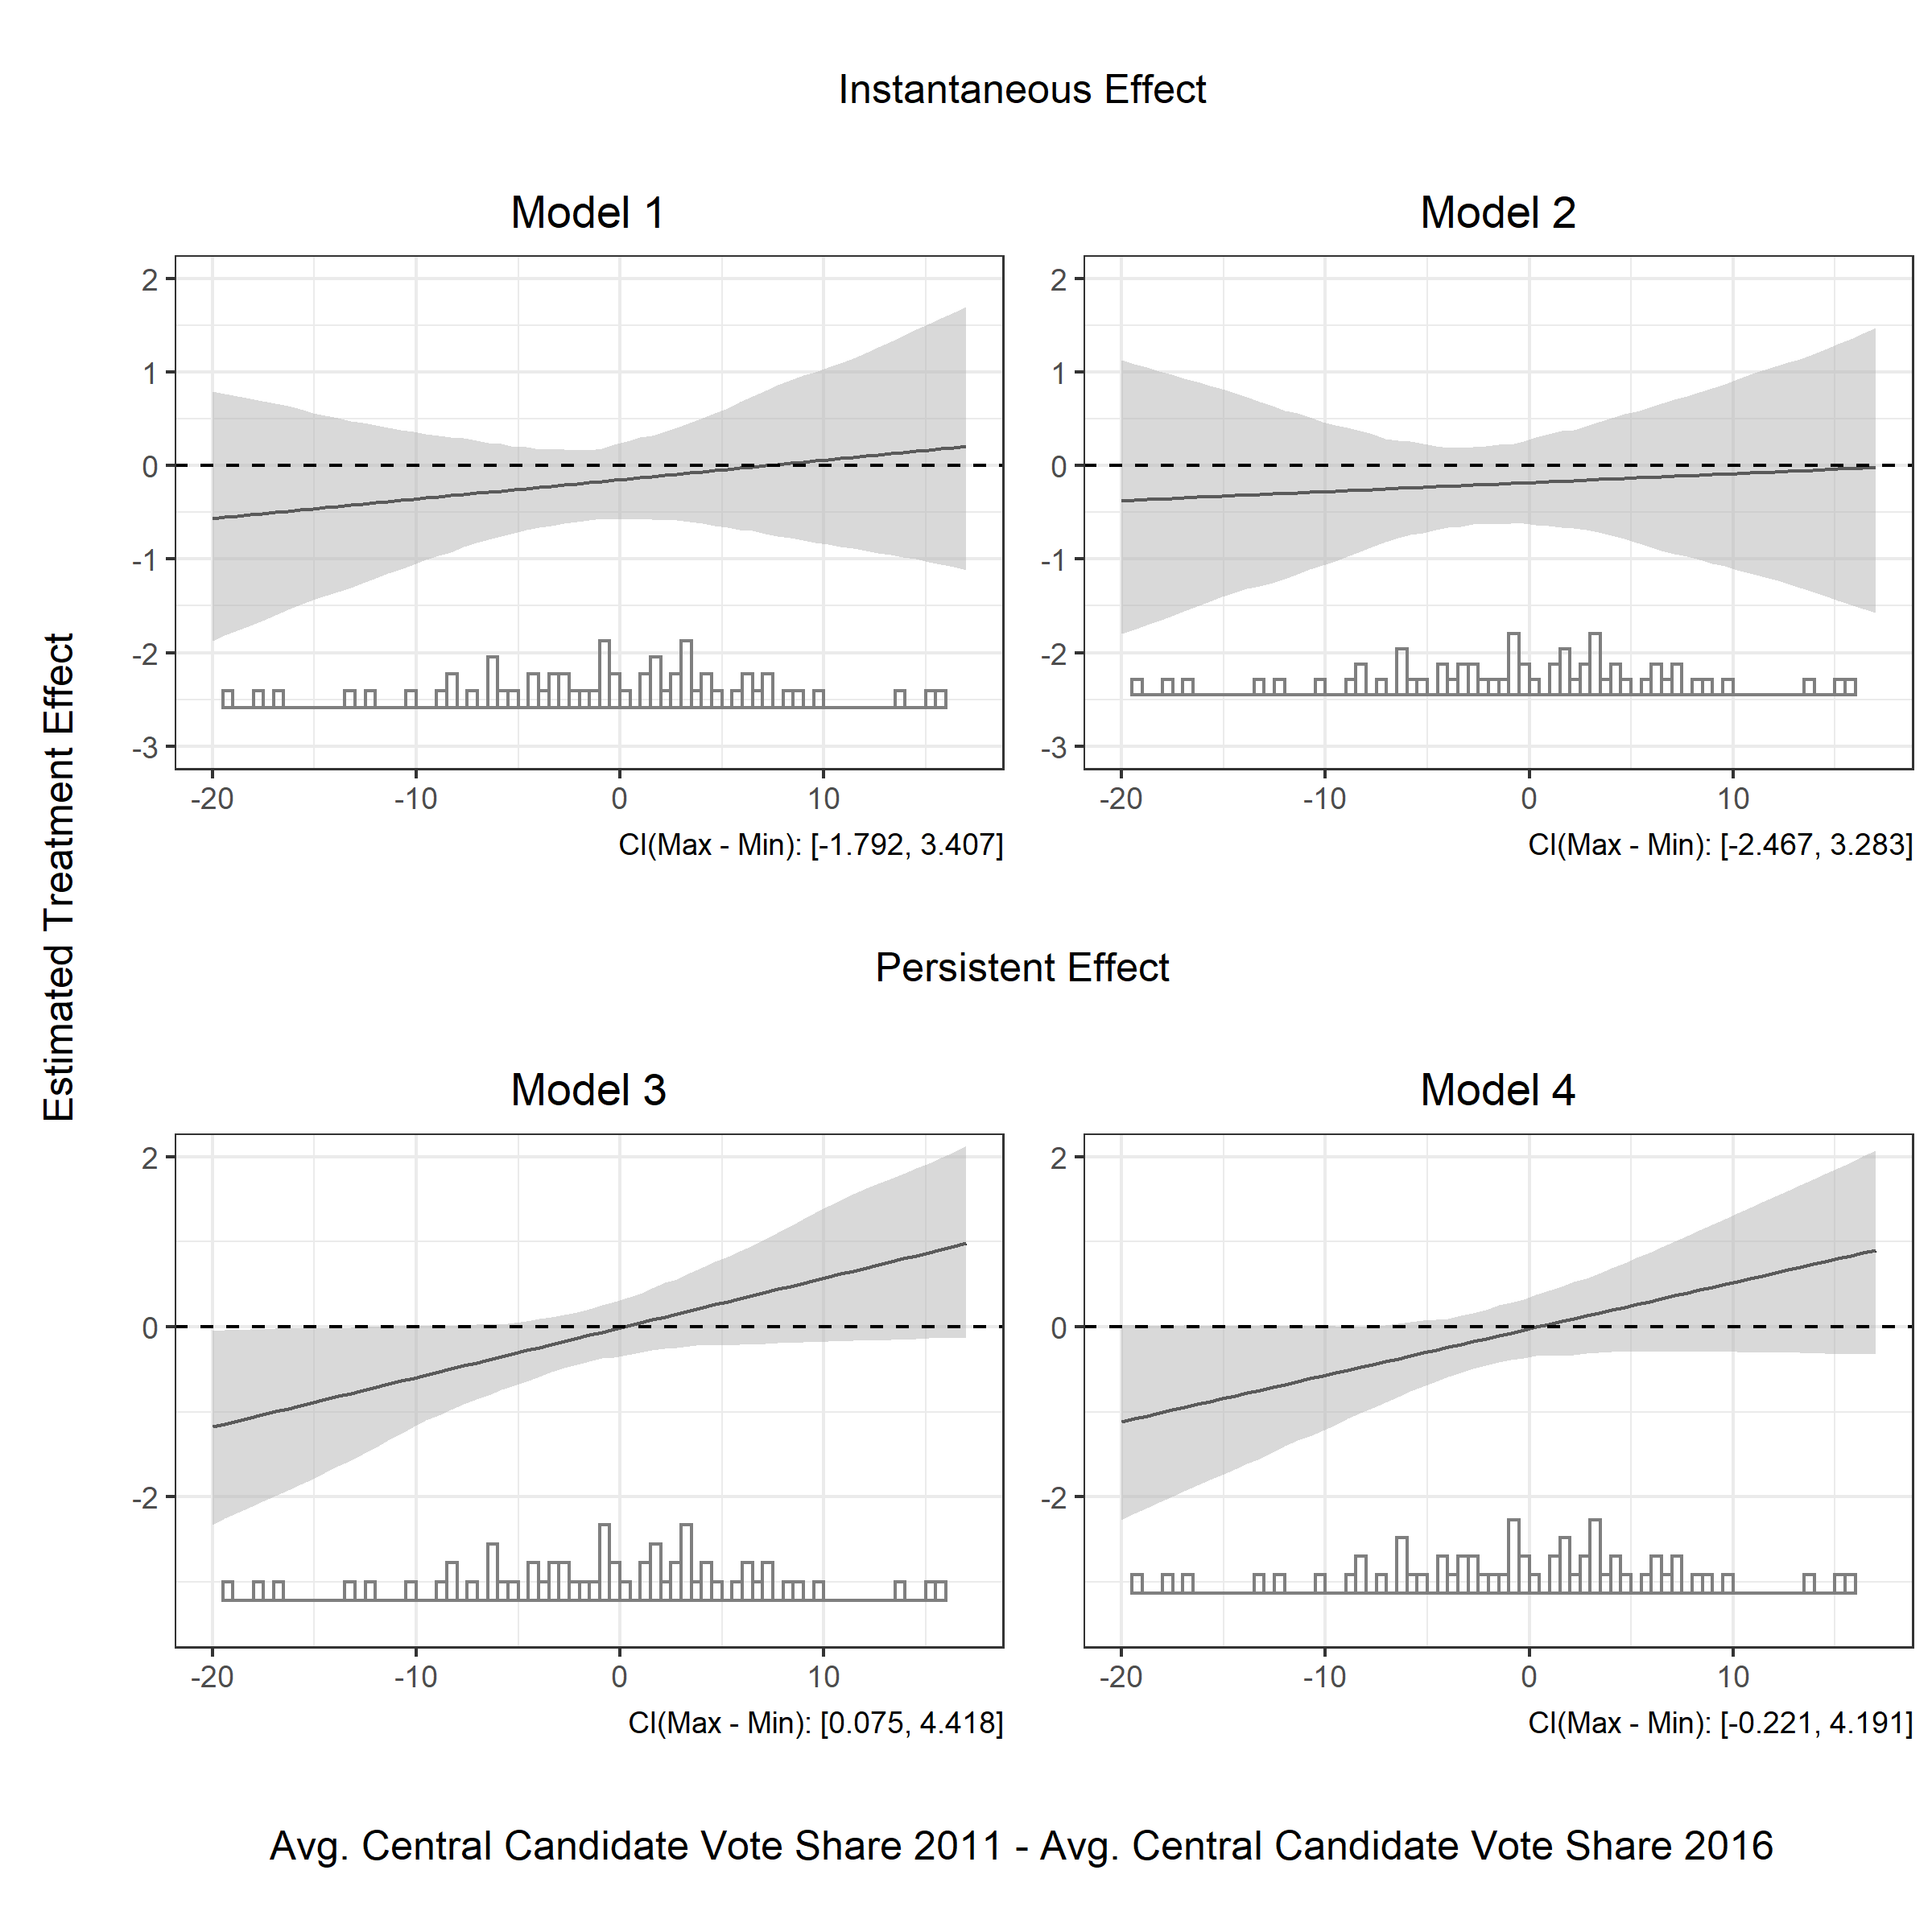
\includegraphics[width=\textwidth]{figure/200218_lfe_share.png}
%	\captionsetup{singlelinecheck=off}
%	\caption[Effect of difference in central candidate vote share]{Estimated non-linear effect of difference in province-level average central candidate vote share across different its different values. Effect estimates are derived from \autoref{tab:lfe_share}. The distributions of calculated difference is displayed as histograms.}
%	\label{fig:lfe_share}
%\end{figure}

\section{Effectiveness of the CPV's placation strategy}
\label{app:repeat}

Although this paper provides an account of the Vietnamese regime's response to what it \textit{believes} has caused the defeats of central candidates in the 2016 VNA election, it does not attempt to verify whether the regime's belief is correct or misguided. This task is nearly impossible, because it would require both a survey of Vietnamese citizens as well as a comprehensive evaluation of provincial officials, which even the Vietnamese state has not been able to do. An alternative, less effective but also less ambitious, way to assess the CPV's inferences, however, is to probe whether it has succeeded in preventing election defeats with its placation strategy.

There are many different reasons the placation strategy could fail to achieve the CPV's goals. First, it is possible that it has misdiagnosed the problem i.e. believing that the local defeats indicate pockets of dissatisfied citizens when they are in fact the product of disloyal or incompetent officials. Second, even if the regime has correctly diagnosed its problem, public dissatisfaction may be more deeply rooted than it has realized and thus cannot be assuaged by a placation strategy. Third, the completely opposite scenario may also be true: if voters are myopic and base their vote choices on short-term considerations, then the effect of the increased transfers may be easily wiped away by immediate events happening to the voters, rendering the former ineffective at shaping vote choice.\fnote{For a comprehensive review of existing works on the question of ``retrospective voting'' in democracies, see \citet{HealyMalhotra2013}.} Finally, the increase in central transfers may create a perverse incentive for citizens to keep voting against central candidates in the future. Given that VNA elections happen only every four to five year and have only become competitive in the last few decades, the CPV may simply have not experienced enough iterations of these elections to learn about all these potential problems.

On the other hand, not all of the above problems may hold true. In particular, strategic voting by voters is less plausible, as it requires voters to both be aware of the CPV's placation strategy and to coordinate to deliver central candidate defeats. In terms of voter awareness, given that this manuscript is--to the best of my knowledge--the first to ever document the CPV's tendency to increase funding to provinces in which it suffered setbacks, and that elections take place not regularly enough and also do so in conjunction with many other important political events such as the national Party Congresses, it is not easy for voters to attribute any improvement in welfare to the results of electoral races in their provinces. This is compounded by the fact that the CPV (perhaps not coincidentally) keeps details of the budget negotiations confidential from the public and never publicly claims credit for central transfers increases, let alone acknowledging that it increased central transfers in response to central candidate defeats in VNA elections. In terms of voter coordination, for a typical electoral district with about $300,000$ voters about $120,000$ must both vote \textit{against} the central candidate for this candidate to have fewer than a 60\% vote share and vote \textit{for} the same local candidate to avoid spreading their votes too thinly. Given the absence of an organized opposition in Vietnam, this level of coordination cannot be expected.

\begin{table}[]
	\centering
	\caption{Table summarizing which provinces had suffered central candidate defeats in each of the 2007, 2011, and 2016 elections}
	\label{tab:defeats}
	\begin{tabular}{lccc}
		\\[-1.8ex]
		\hline
		\hline
		\\[-1.8ex]
		& \multicolumn{3}{c}{Central candidate defeat(s) in…}                                                       \\
		& \multicolumn{1}{l}{2007 election} & \multicolumn{1}{l}{2011 election} & \multicolumn{1}{l}{2016 election} \\ \midrule
		An Giang         & \checkmark  &   &   \\
		Bac Kan          &   & \checkmark  &   \\
		Can Tho          & \checkmark  & \checkmark  & \checkmark  \\
		Dong Thap        &   & \checkmark  & \checkmark  \\
		Hai Duong        &   & \checkmark  &   \\
		Hai Phong        & \checkmark  &   &   \\
		Long An          & \checkmark  & \checkmark  &   \\
		Phu Yen          &   &   & \checkmark  \\
		Soc Trang        &   & \checkmark  & \checkmark  \\
		Tay Ninh         & \checkmark  &   &   \\
		Tra Vinh         &   &   & \checkmark  \\  \midrule	
		Hanoi            & \checkmark & \checkmark  & \checkmark  \\
		Ho Chi Minh City & \checkmark  & \checkmark  & \checkmark  \\ 
		Binh Duong       & \checkmark  & \checkmark  &   \\
		
		\\[-1.8ex]
		\hline
		\hline
		\\[-1.8ex]
	\end{tabular}
\end{table}

To find out whether the remaining concerns could have hampered the CPV's placation strategy, I tabulate central candidate defeats by individual provinces across the last three elections to find out which provinces suffered these defeats in which election and whether these defeats tend to repeat. The data, presented in \autoref{tab:defeats}, conveys a rather nuanced message. Excluding the outlier provinces of Hanoi, Ho Chi Minh City and Binh Duong, in 2011 and 2016 there have been 5 repeated defeats, 6 defeats that were not repeated in the following election, and 6 defeats that did not precede a prior defeat. One province--Can Tho--saw central candidates in all three elections. Three others--Dong Thap, Long An, and Soc Trang--saw two defeats. The remaining six provinces--An Giang, Hai Duong, Hai Phong, Phu Yen, Tay Ninh and Tra Vinh--experienced only one.

At first glance, central candidate defeats do seem to be concentrated in a few provinces: given that the vast majority of provinces have not seen a central candidate defeat in 2007 or 2011, the fact that half of the defeats in 2011 and 2016 happened in the 4 provinces that have suffered one before implies a clear association between past and present defeats.

On the other hand, if the causes behind electoral defeats and victories are somewhat persistent over time, it is not surprising that most Vietnamese provinces would rarely see electoral defeats; after all these defeats are already extremely unlikely given the odds stacked in the central candidates' favor. The more appropriate inference to determine the appropriateness of the placation strategy should therefore be: among provinces that have suffered a central candidate defeat, how likely is another defeat? Here the data in \autoref{tab:defeats} shows a different picture: less than half of the defeats in 2007 and 2011 were repeated in the following election.

\autoref{tab:lfe_repeat} shows the results from a more rigorous treatment that uses three linear fixed effects models applied to province-election year data for the 2011 and 2016 elections. The models aim to use central candidate defeat in the previous election to predict defeat in the present one. In these models, the province fixed effects help control for time-invariant factors unique to each province. They also limit the inference to provinces that have experienced both an election in which a central candidate was defeated and one in which it did not and thus have seen both sides of the CPV's post-election response. The model in Column 1 uses central candidate defeat as the only independent variable. Although not statistically significant (likely due to power issue), the result shows a clear descriptive relationship: all else being equal, provinces that have experienced a central candidate defeat in an election is 28\% less likely to experience another defeat in the following election. 


% Table created by stargazer v.5.2.2 by Marek Hlavac, Harvard University. E-mail: hlavac at fas.harvard.edu
% Date and time: Wed, Sep 16, 2020 - 20:47:02
\begin{table}[!htbp] \centering 
  \caption{Estimated effects of past central candidate defeat and net transfer changes
          on probability of defeat from linear fixed effects models} 
  \label{tab:lfe_repeat} 
\begin{tabular}{@{\extracolsep{5pt}}lccc} 
\\[-1.8ex]\hline 
\hline \\[-1.8ex] 
\\[-1.8ex] & (1) & (2) & (3)\\ 
\hline \\[-1.8ex] 
 Previous Central Candidate Defeat & $-$0.284 & $-$0.292 & $-$0.340 \\ 
  & (0.241) & (0.219) & (0.239) \\ 
  (Logged) Net Transfer Change &  & 0.008 & 0.006 \\ 
  &  & (0.005) & (0.005) \\ 
  Previous Central Candidate Defeat $\times$ \\ (Logged) Net Transfer Change &  &  & 0.011 \\ 
  &  &  & (0.017) \\ 
 \hline \\[-1.8ex] 
Province FEs & Yes & Yes & Yes \\ 
Year FEs & Yes & Yes & Yes \\ 
\hline \\[-1.8ex] 
N & 120 & 120 & 120 \\ 
R$^{2}$ & 0.779 & 0.807 & 0.818 \\ 
\hline 
\hline \\[-1.8ex] 
\multicolumn{4}{l}{$^{*}$p $<$ .1; $^{**}$p $<$ .05; $^{***}$p $<$ .01} \\ 
\end{tabular} 
\end{table} 


Furthermore, in Column 2, to probe the specific effect of central transfers, I add to the model the log of changes in net transfers from the previous election, which is the outcome variable in the main analysis but measured for the previous election. The coefficient is small and indistinguishable from zero, suggesting that changes in net transfers following the previous election have no clear impact on the present election, once the tendency of central candidate defeats to \textit{not} repeat has been accounted for. Another interpretation is that, as long as a province had experienced a central candidate defeats and had received some central transfers from the central government, the exact amount of the transfers no longer matters in determining the outcome of the next election.

In Column 3, I add an interaction term between the two variables; this interaction term would help identify whether changes in net transfers have any particular effect in provinces that have experienced central candidate defeats in the previous election. This conditional effect, obtained by summing the second and third coefficients in Column 3, remains small and indistinguishable from zero. Specifically, the conditional effect estimate is $.017$ and has a 95\% confidence interval of $[-.014,.048]$. The point estimate alone indicates that an increase in net transfers that is equivalent to 1\% of the year-to-year average change would increase the probability of central candidate defeats by 1.7\%, equivalent to $1/20$ of the first coefficient. In other words, provinces that experience central candidate defeats in one election would \textit{not} be more likely to see a repeated defeat unless its net transfers were increased by 20 times of the year-to-year average change. In contrast, the effect estimated in the main manuscript translates equals to only 9.1 times of this amount.

Overall, even though the independent variables in these models are far from exogenous and thus do not allow for strong causal claims, the analysis above and the data from \autoref{tab:defeats} do provide some descriptive statistics to evaluate the CPV's placation strategy. First, it does seem to prevent defeats from repeating, but not to the extent that repeated defeats no longer occur. Second, even though a prior defeat and the subsequent increase to central transfers may help ward off repeated defeats, the exact amount of the transfer increase may not have additional effect at the margin.\fnote{Unfortunately, it is not possible to disentangle the effect of a prior defeat \textit{per se} and that of the increase in transfers that follow.} Third, there is a theoretical possibility that the transfer increase may induce perverse incentive for citizens to keep voting against central candidates, but in practice it may only occur when the size of the increase is impossibly large. Fourth, despite the transfer increases, at least one province still experiences central candidate defeats in every single election, whereas most other provinces that presumably did not receive this treatment have never seen these defeats, suggesting that the problems behind localized defeats may sometimes be too persistent for a placation strategy to fix. Lastly, this strategy is not designed to, and thus understandably has not managed to, prevent new defeats from emerging in provinces that have not seen them before.

Absent data on the size of the problem the CPV is presented with, an assessment of its treatment is never meant to be complete. However, based on data on repeated elections alone, it seems that the strategy of using increased central transfers to placate the voting public has achieved some limited success, although it is unclear that this success is sufficient or sustainable.

\clearpage
%\singlespacing
\inputencoding{utf8}
\printbibliography[heading=bibintoc]


\end{document}


